% fabrication.tex — Part 1 of the build: what to buy, what to cut, and the drawings.
% Build:  python3 tools/make_figures.py && latexmk -lualatex fabrication.tex
\documentclass[10pt]{article}
\newcommand{\doctitle}{Radar build, part 1: parts and fabrication drawings}
% common.tex — shared preamble for the two build documents.
% Compile with LuaLaTeX (fontspec + DejaVu, so Ω µ ° × → print as themselves).
\usepackage[letterpaper,margin=19mm,top=22mm,bottom=20mm,headsep=6mm]{geometry}
\usepackage{fontspec}
\setmainfont{DejaVu Sans}[Scale=0.92]
\setsansfont{DejaVu Sans}[Scale=0.92]
\setmonofont{DejaVu Sans Mono}[Scale=0.86]
\renewcommand{\familydefault}{\sfdefault}
\usepackage{microtype}
\usepackage[table]{xcolor}
\usepackage{graphicx}
\usepackage{tikz}
\usetikzlibrary{arrows.meta,calc,positioning,patterns,decorations.pathreplacing,shapes.geometric,fit,backgrounds}
\usepackage[american,siunitx]{circuitikz}
\usepackage{booktabs,tabularx,longtable,array,multirow,makecell}
\usepackage{enumitem}
\usepackage{titlesec}
\usepackage{fancyhdr}
\usepackage{caption}
\usepackage{pdflscape}
\usepackage[most]{tcolorbox}
\usepackage[hidelinks]{hyperref}
\usepackage{float}

% ── palette (matches the horn build guide and the HFSS guide)
\definecolor{ink}{HTML}{14181D}
\definecolor{muted}{HTML}{5F6670}
\definecolor{rule}{HTML}{C9CDD3}
\definecolor{faint}{HTML}{E3E6EA}
\definecolor{accent}{HTML}{8A3B1E}
\definecolor{boxbg}{HTML}{F4EFE6}
\definecolor{cuout}{HTML}{E2A27A}
\definecolor{cuin}{HTML}{B86F45}
\definecolor{cuedge}{HTML}{6B3A1F}
\definecolor{tabfill}{HTML}{F3D2BC}
\definecolor{bend}{HTML}{1F5F8B}
\definecolor{dimc}{HTML}{3B4450}
\definecolor{wood}{HTML}{D9B98C}
\definecolor{woodedge}{HTML}{8C6A3F}
\definecolor{alu}{HTML}{B8C0C8}
\definecolor{rfmod}{HTML}{CFE0EE}
\definecolor{pcb}{HTML}{CFE3CF}
\definecolor{sig}{HTML}{2E7D32}
\definecolor{pwr}{HTML}{C62828}
\definecolor{logic}{HTML}{1565C0}
\definecolor{okgreen}{HTML}{2E7D32}
\definecolor{warnamber}{HTML}{B26A00}
\color{ink}

% ── headings
\titleformat{\section}{\Large\bfseries\color{ink}}{\color{accent}\thesection}{0.7em}{}
\titleformat{\subsection}{\large\bfseries\color{accent}}{\thesubsection}{0.6em}{}
\titleformat{\subsubsection}{\normalsize\bfseries\color{ink}}{}{0em}{}
\titlespacing*{\section}{0pt}{2pt}{8pt}
\titlespacing*{\subsection}{0pt}{12pt}{4pt}
\titlespacing*{\subsubsection}{0pt}{8pt}{2pt}
\setlength{\parindent}{0pt}
\setlength{\parskip}{5pt}
\linespread{1.08}
\setlist{itemsep=2pt,topsep=3pt,leftmargin=16pt}
\captionsetup{font={small,color=muted},labelfont={bf,color=muted},justification=raggedright,singlelinecheck=false,skip=4pt}

% ── tables
\renewcommand{\arraystretch}{1.25}
\arrayrulecolor{rule}
\newcolumntype{L}{>{\raggedright\arraybackslash}X}
\newcolumntype{P}[1]{>{\raggedright\arraybackslash}p{#1}}

% ── callouts
\newtcolorbox{note}[1][]{enhanced,colback=boxbg,colframe=boxbg,borderline west={2.4pt}{0pt}{accent},
  arc=0pt,left=8pt,right=8pt,top=4pt,bottom=4pt,fonttitle=\bfseries,coltitle=ink,
  title={#1},attach title to upper={\par\smallskip},before skip=6pt,after skip=8pt}
\newtcolorbox{warn}[1][]{enhanced,colback=warnamber!8,colframe=warnamber!8,borderline west={2.4pt}{0pt}{warnamber},
  arc=0pt,left=8pt,right=8pt,top=4pt,bottom=4pt,fonttitle=\bfseries,coltitle=warnamber!80!black,
  title={#1},attach title to upper={\par\smallskip},before skip=6pt,after skip=8pt}
\newtcolorbox{okbox}{enhanced,colback=okgreen!7,colframe=okgreen!7,borderline west={2.4pt}{0pt}{okgreen},
  arc=0pt,left=8pt,right=8pt,top=4pt,bottom=4pt,before skip=4pt,after skip=8pt}
\newcommand{\checkline}[1]{\begin{okbox}\textbf{\color{okgreen!70!black}Check.}\ #1\end{okbox}}

% ── a numbered step banner
\newcounter{stepno}
\newcommand{\step}[1]{\stepcounter{stepno}\par\smallskip
  \noindent\begin{tikzpicture}[baseline=(t.base)]
    \node[fill=accent,text=white,font=\bfseries,minimum width=7mm,minimum height=6mm,inner sep=2pt](n){\thestepno};
    \node[right=3mm of n.east,anchor=west,font=\large\bfseries](t){#1};
  \end{tikzpicture}\par\nopagebreak\smallskip}

% ── TikZ styles for drawings
\tikzset{
  cut/.style={draw=cuedge,line width=0.6pt,line join=round},
  wall/.style={cut,fill=cuout},
  tab/.style={cut,fill=tabfill},
  fold/.style={draw=bend,line width=0.6pt,dash pattern=on 3pt off 2pt},
  centre/.style={draw=muted,line width=0.35pt,dash pattern=on 6pt off 2pt on 1pt off 2pt},
  dim/.style={draw=dimc,line width=0.35pt,{Stealth[length=1.6mm,width=1.1mm]}-{Stealth[length=1.6mm,width=1.1mm]}},
  ext/.style={draw=dimc,line width=0.25pt},
  dimlabel/.style={midway,sloped,fill=white,inner sep=0.8pt,font=\scriptsize,text=dimc},
  partlabel/.style={font=\bfseries\large,text=accent},
  callout/.style={draw=muted,line width=0.35pt},
  woodpart/.style={draw=woodedge,line width=0.6pt,fill=wood},
  alupart/.style={draw=black!60,line width=0.6pt,fill=alu},
  module/.style={draw=black!65,line width=0.5pt,fill=rfmod,rounded corners=0.6pt},
  hidden/.style={draw=muted,line width=0.4pt,dash pattern=on 2pt off 1.5pt},
  coax/.style={draw=black!80,line width=1.1pt,rounded corners=2pt},
}

% ── a scale bar and a print-check square for the 1:1 templates
\newcommand{\checksquare}{%
  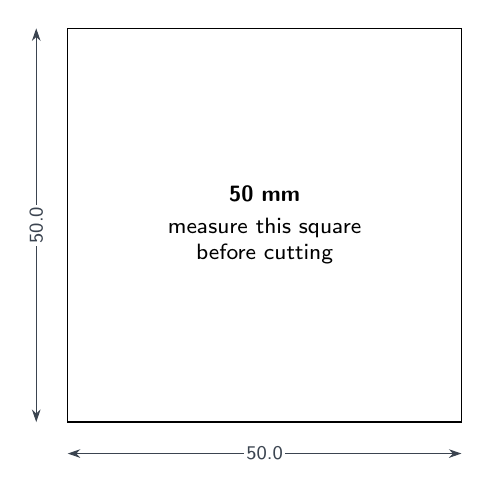
\begin{tikzpicture}[x=1mm,y=1mm]
    \draw[line width=0.5pt] (0,0) rectangle (50,50);
    \node[align=center,font=\footnotesize] at (25,25) {\textbf{50 mm}\\[2pt]measure this square\\before cutting};
    \draw[dim] (0,-4) -- (50,-4) node[dimlabel]{50.0};
    \draw[dim] (-4,0) -- (-4,50) node[dimlabel]{50.0};
  \end{tikzpicture}}

\newcommand{\code}[1]{\texttt{#1}}
\newcommand{\fig}[1]{Figure~\ref{#1}}

% ── running header and footer
\pagestyle{fancy}
\fancyhf{}
\renewcommand{\headrulewidth}{0.4pt}
\renewcommand{\headrule}{\hbox to\headwidth{\color{rule}\leaders\hrule height \headrulewidth\hfill}}
\fancyhead[L]{\footnotesize\color{muted}\doctitle}
\fancyhead[R]{\footnotesize\color{muted}radar-dev · 2.4 GHz FMCW radar}
\fancyfoot[L]{\footnotesize\color{muted}Sizes in mm unless marked. Generated from antenna/tools/horn.py and the 3-D model.}
\fancyfoot[R]{\footnotesize\color{muted}\thepage}
\fancypagestyle{plain}{\fancyhf{}\fancyfoot[R]{\footnotesize\color{muted}\thepage}\renewcommand{\headrulewidth}{0pt}}

% generated by tools/make_figures.py — do not edit
\newcommand{\aperW}{263.8}
\newcommand{\aperH}{193.1}
\newcommand{\pipeW}{86.4}
\newcommand{\pipeH}{43.2}
\newcommand{\flareL}{91.5}
\newcommand{\pipeL}{115}
\newcommand{\probeZ}{43.7}
\newcommand{\probeLen}{28}
\newcommand{\rodCut}{32}
\newcommand{\seam}{147.9}
\newcommand{\hTop}{118.3}
\newcommand{\hSide}{127.5}
\newcommand{\wideW}{87.5}
\newcommand{\backW}{88.5}
\newcommand{\backH}{44.3}
\newcommand{\tabW}{6}
\newcommand{\gain}{13.4}
\newcommand{\hpE}{34.2}
\newcommand{\hpH}{36.2}
\newcommand{\boardW}{457}
\newcommand{\boardD}{381}
\newcommand{\upH}{530.8}
\newcommand{\upX}{213}
\newcommand{\upCC}{426}
\newcommand{\beamLen}{444}
\newcommand{\beamRXlen}{408}
\newcommand{\beamRXtop}{252.8}
\newcommand{\beamTXtop}{542.8}
\newcommand{\rxY}{300}
\newcommand{\txY}{590}
\newcommand{\hornBase}{193.1}
\newcommand{\rowGap}{26.2}
\newcommand{\braceLen}{242.2}
\newcommand{\saddleW}{56.2}
\newcommand{\saddleGap}{48.2}
\newcommand{\saddleD}{34}
\newcommand{\saddleH}{32}
\newcommand{\saddleBehind}{90}
\newcommand{\overhang}{36}
\newcommand{\screenW}{293.1}
\newcommand{\screenH}{130}
\newcommand{\braceFootX}{128}
\newcommand{\txTop}{721.9}
\newcommand{\frontToFrame}{145.5}
\newcommand{\beamRXbottom}{240.8}
\newcommand{\braceTop}{226.8}
\newcommand{\leanTop}{39}
\newcommand{\leanSide}{44}
\newcommand{\cornerBend}{64}
\newcommand{\braceAngle}{69}
\newcommand{\sheetPct}{62}
\newcommand{\sheetIn}{178}

% table rows from a file: the primitive \input, because LaTeX's is not expandable inside a tabular
\makeatletter\newcommand{\rowsfrom}[1]{\@@input generated/#1.tex }\makeatother
\newcolumntype{Y}{>{\centering\arraybackslash}X}

\graphicspath{{generated/}{../breadboard/assembly/steps/}{../3d/renders/radar-bench/}}
\newcommand{\partsMissing}{21}


\begin{document}

% ───────────────────────────────────────────────────────────── title page
\thispagestyle{plain}
\begin{tikzpicture}[remember picture,overlay]
  \fill[accent] (current page.north west) rectangle ([yshift=-9mm]current page.north east);
\end{tikzpicture}
\vspace*{6mm}
{\color{muted}\small radar-dev \quad·\quad 2.4 GHz FMCW radar \quad·\quad part 1 of 2}\par
\vspace{2mm}
{\fontsize{26}{30}\selectfont\bfseries Parts and fabrication\par}
\vspace{1mm}
{\Large\color{accent} Everything to buy, cut and drill, drawn to scale\par}
\vspace{5mm}
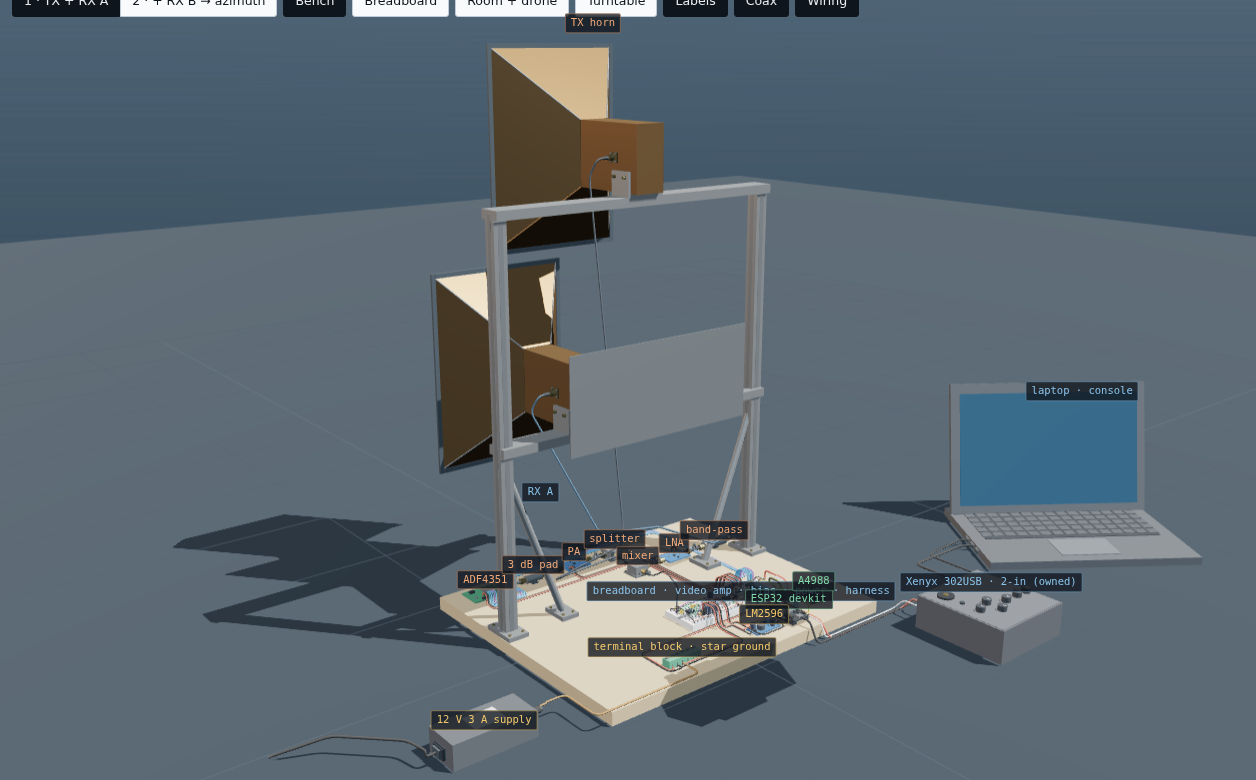
\includegraphics[width=\linewidth]{bench_view.png}\par
{\footnotesize\color{muted} The finished bench, from the 3-D model (\code{3d/radar-bench.html}). Every size in this document comes from that model and from the horn solver, not from hand.}
\vspace{4mm}

\begin{minipage}[t]{0.48\linewidth}
\textbf{This document} says what every part is, how big it is, and how much to buy:
\begin{itemize}
  \item the parts list, checked against your order
  \item full-size cutting templates for the copper horns
  \item the frame, with every cut and hole
  \item cable runs, schematics, and the breadboard layout
\end{itemize}
\end{minipage}\hfill
\begin{minipage}[t]{0.48\linewidth}
\textbf{Part 2, the assembly guide,} uses these parts to put it together in order, with a check at the end of every stage, ending with the radar seeing someone walk across the room.

\smallskip
{\color{muted}\small Sizes are millimetres unless marked. Print the template pages at \textbf{100\,\%, “actual size”}, never “fit to page”, and measure the 50\,mm square on each one before cutting.}
\end{minipage}

\newpage
\tableofcontents
\newpage

% ───────────────────────────────────────────────────────────── 1 overview
\section{The system on one page}\label{sec:overview}

The radar sends out a tone that sweeps steadily up from 2400 to 2483.5\,MHz, then listens for echoes. An echo from something far away was sent earlier, so it comes back at a slightly lower pitch than what is being sent right now. Mixing the two together gives a low beat tone whose pitch says how far away the thing is. A sound card records that tone and the laptop turns pitch into distance.

\begin{figure}[H]
\centering
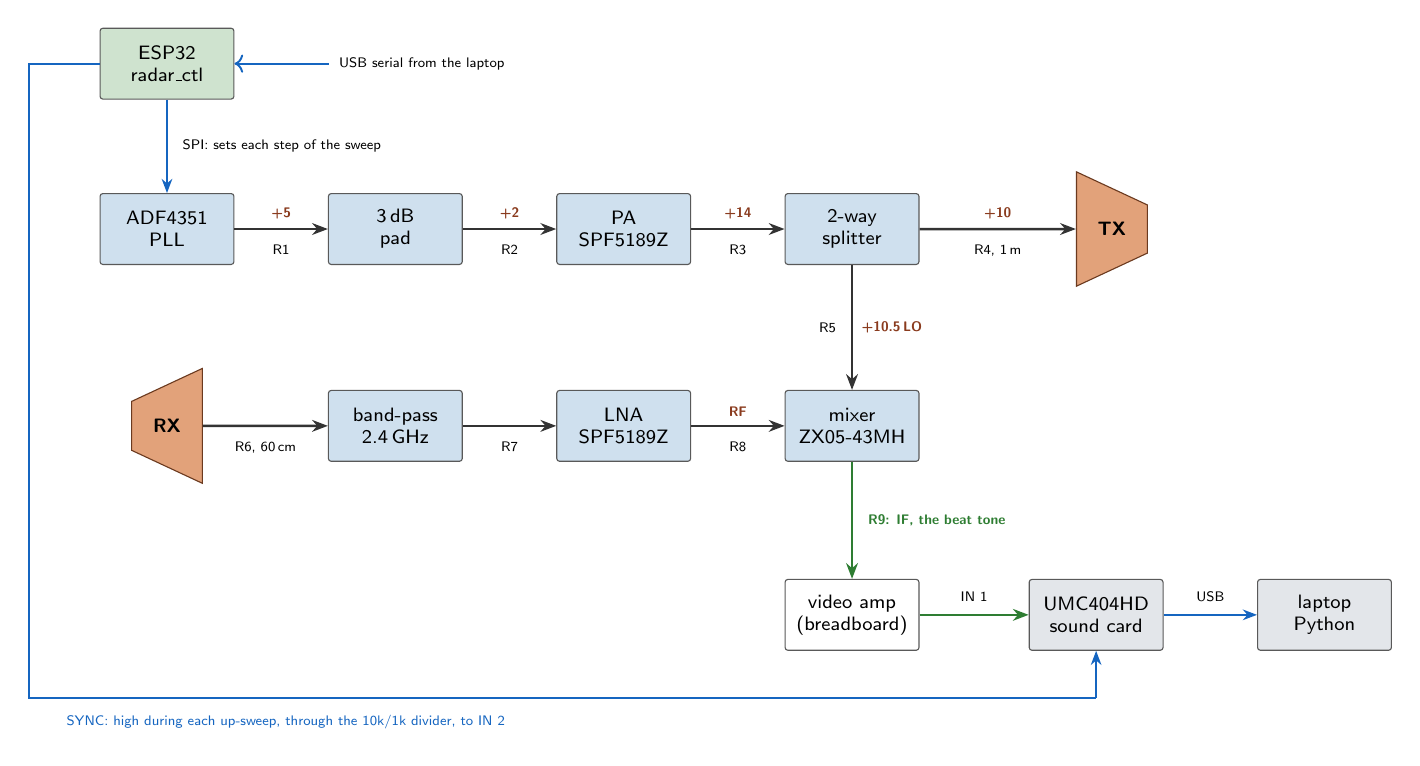
\begin{tikzpicture}[
  blk/.style={draw=black!65,fill=rfmod,rounded corners=1pt,minimum height=9mm,minimum width=17mm,align=center,font=\scriptsize},
  dig/.style={blk,fill=pcb},
  bb/.style={blk,fill=white},
  ant/.style={draw=cuedge,fill=cuout,minimum height=9mm,minimum width=12mm,align=center,font=\scriptsize\bfseries,trapezium,trapezium angle=65,shape border rotate=270},
  rf/.style={draw=black!80,line width=0.9pt,-{Stealth[length=2mm]}},
  ifl/.style={draw=sig,line width=0.9pt,-{Stealth[length=2mm]}},
  lg/.style={draw=logic,line width=0.7pt,-{Stealth[length=1.8mm]}},
  lvl/.style={font=\tiny\bfseries,text=accent,fill=white,inner sep=1pt},
  ]
  \node[dig] (esp) at (0,2.1) {ESP32\\radar\_ctl};
  \node[blk] (adf) at (0,0) {ADF4351\\PLL};
  \node[blk] (pad) at (2.9,0) {3\,dB\\pad};
  \node[blk] (pa)  at (5.8,0) {PA\\SPF5189Z};
  \node[blk] (spl) at (8.7,0) {2-way\\splitter};
  \node[ant] (tx)  at (12.0,0) {TX};
  \node[ant,shape border rotate=90] (rx) at (0,-2.5) {RX};
  \node[blk] (bpf) at (2.9,-2.5) {band-pass\\2.4\,GHz};
  \node[blk] (lna) at (5.8,-2.5) {LNA\\SPF5189Z};
  \node[blk] (mix) at (8.7,-2.5) {mixer\\ZX05-43MH};
  \node[bb]  (amp) at (8.7,-4.9) {video amp\\(breadboard)};
  \node[blk,fill=faint] (snd) at (11.8,-4.9) {UMC404HD\\sound card};
  \node[blk,fill=faint] (pc)  at (14.7,-4.9) {laptop\\Python};
  \draw[rf] (adf) -- node[lvl,above=2pt]{+5} node[font=\tiny,below=2pt]{R1} (pad);
  \draw[rf] (pad) -- node[lvl,above=2pt]{+2} node[font=\tiny,below=2pt]{R2} (pa);
  \draw[rf] (pa)  -- node[lvl,above=2pt]{+14} node[font=\tiny,below=2pt]{R3} (spl);
  \draw[rf] (spl) -- node[lvl,above=2pt]{+10} node[font=\tiny,below=2pt]{R4, 1\,m} (tx);
  \draw[rf] (spl) -- node[lvl,right=2pt]{+10.5\,LO} node[font=\tiny,left=2pt]{R5} (mix);
  \draw[rf] (rx)  -- node[font=\tiny,below=2pt]{R6, 60\,cm} (bpf);
  \draw[rf] (bpf) -- node[font=\tiny,below=2pt]{R7} (lna);
  \draw[rf] (lna) -- node[font=\tiny,below=2pt]{R8} node[lvl,above=2pt]{RF} (mix);
  \draw[ifl] (mix) -- node[font=\tiny\bfseries,text=sig,right=2pt]{R9: IF, the beat tone} (amp);
  \draw[ifl] (amp) -- node[font=\tiny,above=1pt]{IN 1} (snd);
  \draw[lg] (snd) -- node[font=\tiny,above=1pt]{USB} (pc);
  \draw[lg] (esp) -- node[font=\tiny,right=2pt]{SPI: sets each step of the sweep} (adf);
  \draw[draw=logic,line width=0.7pt] (esp.west) -- ++(-0.9,0) |- ([yshift=-6mm]snd.south) coordinate(sb);
  \draw[lg] (sb) -- (snd.south);
  \node[font=\tiny,text=logic,anchor=north west] at (-1.4,-6.05) {SYNC: high during each up-sweep, through the 10k/1k divider, to IN 2};
  \draw[lg,<-] (esp.east) -- ++(1.2,0) node[right,font=\tiny,align=left]{USB serial from the laptop};
\end{tikzpicture}
\caption{The signal path. Thick black arrows are coax (SMA cables); numbers in red are the signal strength in dBm at that point. Green is the low-frequency beat tone; blue is logic.}
\end{figure}

\begin{minipage}[t]{0.5\linewidth}
\begin{tabular}{@{}P{0.40\linewidth}P{0.52\linewidth}@{}}
\toprule
\textbf{what} & \textbf{value} \\ \midrule
sweep & 2400–2483.5\,MHz, the whole 2.4\,GHz ISM band \\
sweep timing & 64 steps in 6.4\,ms, repeats every 7.4\,ms \\
distance resolution & 1.80\,m per range cell \\
speed resolution & 0.13\,m/s \\
transmit power & about +10\,dBm into a \gain\,dBi horn \\
\bottomrule
\end{tabular}
\end{minipage}\hfill
\begin{minipage}[t]{0.47\linewidth}
\begin{tabular}{@{}P{0.40\linewidth}P{0.52\linewidth}@{}}
\toprule
\textbf{what} & \textbf{value} \\ \midrule
horns & 3 copper pyramidal horns, \aperW\,×\,\aperH\ mouth \\
beam & about \hpE°\,×\,\hpH° \\
beat amplifier & gain 1111 (61\,dB), cut-off 15.9\,kHz \\
power in & 12\,V, 3\,A supply \\
footprint & \boardW\,×\,\boardD\ plywood, \txTop\ tall \\
\bottomrule
\end{tabular}
\end{minipage}

\enlargethispage{2\baselineskip}
\subsection*{The four things you build}
\begin{enumerate}
  \item \textbf{Three copper horns} (section \ref{sec:horn}). Two face out as transmitter and receiver; the third is for the second receiver later (stage 2), and is built now so the two receivers come out as twins.
  \item \textbf{The frame} (section \ref{sec:frame}). A plywood board with two uprights and two cross beams. The transmit horn sits on the top beam, the receive horn and an empty bay on the lower one.
  \item \textbf{The RF chain} (section \ref{sec:rf}). Seven bought modules screwed to the board and joined with SMA cables. Nothing to make, but the cable runs matter.
  \item \textbf{The breadboard} (section \ref{sec:bb}). The beat-tone amplifier, the power distribution and the logic wiring. Two op-amps and about sixty parts, no soldering.
\end{enumerate}

\newpage
% ───────────────────────────────────────────────────────────── 2 parts list
\section{What to buy}\label{sec:parts}

Every part the build needs. The last column is checked against your order spreadsheet (\code{BOM\_Radar\_Build.xlsx}): \textbf{\partsMissing\ lines are not on it}. Most of those are cheap and easy to get, or you already have them; the three you cannot work around are marked in the box below.

\begin{warn}[Not on your list, and the build stops without them]
\textbf{The two long SMA cables} (R4, about 1\,m, splitter up to the transmit horn; R6, about 60\,cm, receive horn down to the band-pass filter). The 20\,cm jumpers you ordered cannot reach the horns, which sit 30 and 60\,cm above the board. \textbf{The ESP32 and the two TL072 op-amps}: without them nothing sweeps and nothing is amplified. Check also that you have \textbf{two} SPF5189Z modules (the PA and the LNA are the same part) and \textbf{three} copper sheets.
\end{warn}

{\small
\begin{longtable}{@{}P{0.27\linewidth}P{0.075\linewidth}P{0.41\linewidth}P{0.165\linewidth}@{}}
\toprule
\textbf{part} & \textbf{qty} & \textbf{what it is, what it does} & \textbf{your order} \\ \midrule
\endfirsthead
\toprule
\textbf{part} & \textbf{qty} & \textbf{what it is, what it does} & \textbf{your order} \\ \midrule
\endhead
\bottomrule
\endfoot
\rowsfrom{parts_rows}
\end{longtable}}

\subsection{Your order, as it stands}
For reference, the spreadsheet as read. Lines with no price are ones the sheet leaves blank.

{\small
\begin{longtable}{@{}P{0.6\linewidth}P{0.15\linewidth}@{}}
\toprule
\textbf{line in BOM\_Radar\_Build.xlsx} & \textbf{price} \\ \midrule
\endhead
\rowsfrom{order_rows}
\bottomrule
\end{longtable}}

\subsection{Tools}\label{sec:tools}
{\small
\begin{tabularx}{\linewidth}{@{}P{0.38\linewidth}L@{}}
\toprule
\textbf{tool} & \textbf{used for} \\ \midrule
aviation snips or a sheet nibbler & cutting the copper \\
steel rule, square, fine marker or scriber & marking out \\
60–100\,W soldering iron with a big tip, or a small gas torch & the horn seams. A 25\,W electronics iron cannot heat the sheet \\
small electronics iron, 25–40\,W & header pins, the IF pigtail, the probe into the SMA cup \\
two lengths of angle iron or hardwood, and clamps & folding tabs on a straight line \\
drill with 2.7, 3.5, 4.5 and 2\,mm bits; centre punch; files & connector holes, screw clearances, pilot holes, deburring \\
hand saw and a mitre box or square & the uprights, beams and braces \\
calipers (digital) & every horn size, and the probe \\
multimeter & seams, rails, the buck converter's 5.00\,V \\
8\,mm (5/16\,in) SMA spanner, or a small adjustable & SMA nuts: finger tight, then 1/8 turn \\
flush snips, wire strippers, tweezers & the breadboard \\
laptop with Arduino IDE (ESP32 core) and Python 3 & the firmware and the radar software \\
gloves and safety glasses; ventilation & cut copper is sharp; flux fumes \\
\textit{nice to have:} a VNA that reaches 2.5\,GHz & measuring the horns' match. Borrow one for twenty minutes \\
\bottomrule
\end{tabularx}}

\newpage
% ───────────────────────────────────────────────────────────── 3 the horns
\section{The copper horns}\label{sec:horn}

Each horn is a rectangular pipe with a flared mouth, made from nine flat pieces of 24\,gauge copper soldered along folded tabs. The pipe is \pipeW\,×\,\pipeH\ inside and \pipeL\ long; the flare opens to \aperW\,×\,\aperH\ over \flareL. A brass rod pushed through the pipe wall from an SMA connector is the feed. Make three, identical.

\begin{figure}[H]
\centering
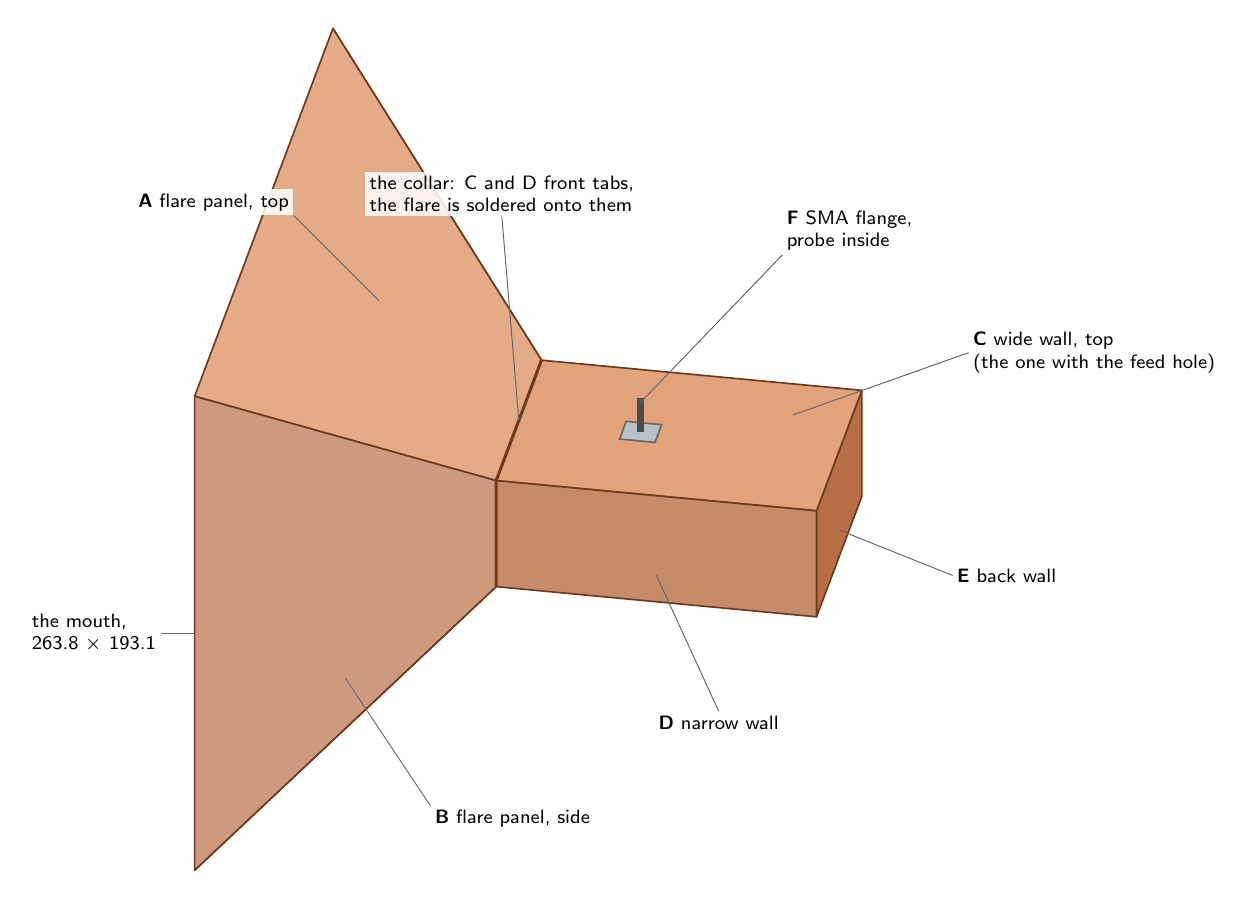
\begin{tikzpicture}[x=0.36mm,y=0.36mm]
\path[draw=cuedge,line width=0.6pt,line join=round,fill=cuin!80!black] (-105.02,13.19) -- (-105.02,50.59) -- (-178.59,167.60) -- (-178.59,0.39) -- cycle;
\path[draw=cuedge,line width=0.6pt,line join=round,fill=cuin!80!black] (-105.02,13.19) -- (-121.01,-29.30) -- (-227.38,-129.35) -- (-178.59,0.39) -- cycle;
\path[draw=cuedge,line width=0.6pt,line join=round,fill=cuin] (7.99,2.55) -- (-7.99,-39.95) -- (-7.99,-2.55) -- (7.99,39.95) -- cycle;
\path[draw=cuedge,line width=0.6pt,line join=round,fill=cuout] (7.99,39.95) -- (-7.99,-2.55) -- (-121.01,8.10) -- (-105.02,50.59) -- cycle;
\path[draw=cuedge,line width=0.6pt,line join=round,fill=cuout!90] (-105.02,50.59) -- (-121.01,8.10) -- (-227.38,37.86) -- (-178.59,167.60) -- cycle;
\path[draw=cuedge,line width=0.6pt,line join=round,fill=cuin!80] (-7.99,-39.95) -- (-7.99,-2.55) -- (-121.01,8.10) -- (-121.01,-29.30) -- cycle;
\path[draw=cuedge,line width=0.6pt,line join=round,fill=cuin!70] (-121.01,-29.30) -- (-121.01,8.10) -- (-227.38,37.86) -- (-227.38,-129.35) -- cycle;
\path[draw=cuedge,line width=1.1pt] (-105.02,50.59) -- (-121.01,8.10) -- (-121.01,-29.30);
\path[alupart] (-62.65,27.84) -- (-65.00,21.59) -- (-77.48,22.77) -- (-75.14,29.01) -- cycle;
\path[draw=black!70,line width=2.4pt] (-70.07,25.30) -- (-70.07,37.42);
\draw[callout] (-162.50,71.66) -- (-192.50,101.66) node[anchor=south east,font=\scriptsize,align=left,fill=white,fill opacity=0.85,text opacity=1,inner sep=1.5pt] {\textbf{A} flare panel, top};
\draw[callout] (-227.38,-45.75) -- (-239.38,-45.75) node[anchor=east,font=\scriptsize,align=left,fill=white,fill opacity=0.85,text opacity=1,inner sep=1.5pt] {the mouth,\\263.8 × 193.1};
\draw[callout] (-174.19,-61.62) -- (-144.19,-106.62) node[anchor=north west,font=\scriptsize,align=left,fill=white,fill opacity=0.85,text opacity=1,inner sep=1.5pt] {\textbf{B} flare panel, side};
\draw[callout] (-113.02,29.35) -- (-119.02,101.35) node[anchor=south,font=\scriptsize,align=left,fill=white,fill opacity=0.85,text opacity=1,inner sep=1.5pt] {the collar: C and D front tabs,\\the flare is soldered onto them};
\draw[callout] (-70.07,35.69) -- (-20.07,87.69) node[anchor=south west,font=\scriptsize,align=left,fill=white,fill opacity=0.85,text opacity=1,inner sep=1.5pt] {\textbf{F} SMA flange,\\probe inside};
\draw[callout] (-16.35,31.24) -- (45.65,53.24) node[anchor=west,font=\scriptsize,align=left,fill=white,fill opacity=0.85,text opacity=1,inner sep=1.5pt] {\textbf{C} wide wall, top\\(the one with the feed hole)};
\draw[callout] (0.00,-9.35) -- (40.00,-25.35) node[anchor=west,font=\scriptsize,align=left,fill=white,fill opacity=0.85,text opacity=1,inner sep=1.5pt] {\textbf{E} back wall};
\draw[callout] (-64.50,-25.27) -- (-42.50,-73.27) node[anchor=north,font=\scriptsize,align=left,fill=white,fill opacity=0.85,text opacity=1,inner sep=1.5pt] {\textbf{D} narrow wall};
\end{tikzpicture}

\caption{One horn seen from behind and above, as it comes off the bench before it is rolled onto its side for mounting. There are two each of A, B, C and D, and one E. The bottom C has no hole.}
\end{figure}

{\small
\begin{tabularx}{\linewidth}{@{}p{8mm}P{0.24\linewidth}p{9mm}LP{0.2\linewidth}@{}}
\toprule
\textbf{piece} & \textbf{name} & \textbf{qty} & \textbf{the wall itself (tabs extra)} & \textbf{folds} \\ \midrule
A & flare panel, top and bottom & 2 & trapezoid, edges \pipeW\ and \aperW, \hTop\ high & none \\
B & flare panel, sides & 2 & trapezoid, edges \pipeH\ and \aperH, \hSide\ high; tabs on both slanted edges & \cornerBend° \\
C & pipe wall, wide & 2 & \wideW\,×\,\pipeL; tabs on both long edges and the front & 90° sides, \leanTop° front \\
D & pipe wall, narrow & 2 & \pipeH\,×\,\pipeL; tab on the front edge & \leanSide° front \\
E & back wall & 1 & \backW\,×\,\backH; tabs on all four edges, corners notched & 90° \\
F & SMA flange and probe & 1 & bought; brass rod cut \rodCut, trimmed to \probeLen\ inside & — \\
\bottomrule
\end{tabularx}}

\smallskip
Every tab is \tabW\,mm wide. The slanted edges of A and B must both come out \seam\,mm, because that is where they meet; if they differ the flare will not close. C and E are cut a little over the pipe's \pipeW\ because the sheet is 0.53\,mm thick and they lap over the other walls: the inside still comes out \pipeW\,×\,\pipeH.

\begin{figure}[H]
\centering\footnotesize
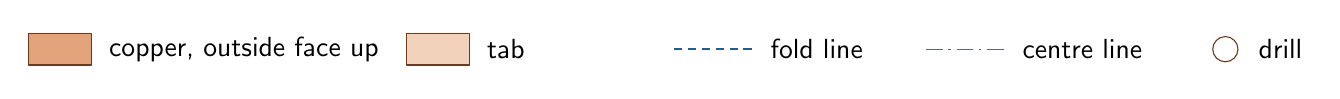
\begin{tikzpicture}[x=1mm,y=1mm]
  \path[wall] (0,0) rectangle (8,4); \node[right] at (9,2) {copper, outside face up};
  \path[tab] (48,0) rectangle (56,4); \node[right] at (57,2) {tab};
  \path[fold] (82,2) -- (92,2); \node[right] at (93,2) {fold line};
  \path[centre] (114,2) -- (124,2); \node[right] at (125,2) {centre line};
  \draw[cuedge,fill=white] (152,2) circle (1.6); \node[right] at (155,2) {drill};
\end{tikzpicture}
\end{figure}

\newpage
\subsection{The flare panels, flat}
Drawn to scale (1\,:\,2), each as seen from its outside face. The long edge is the mouth; the short edge meets the pipe.

\begin{figure}[H]
\centering
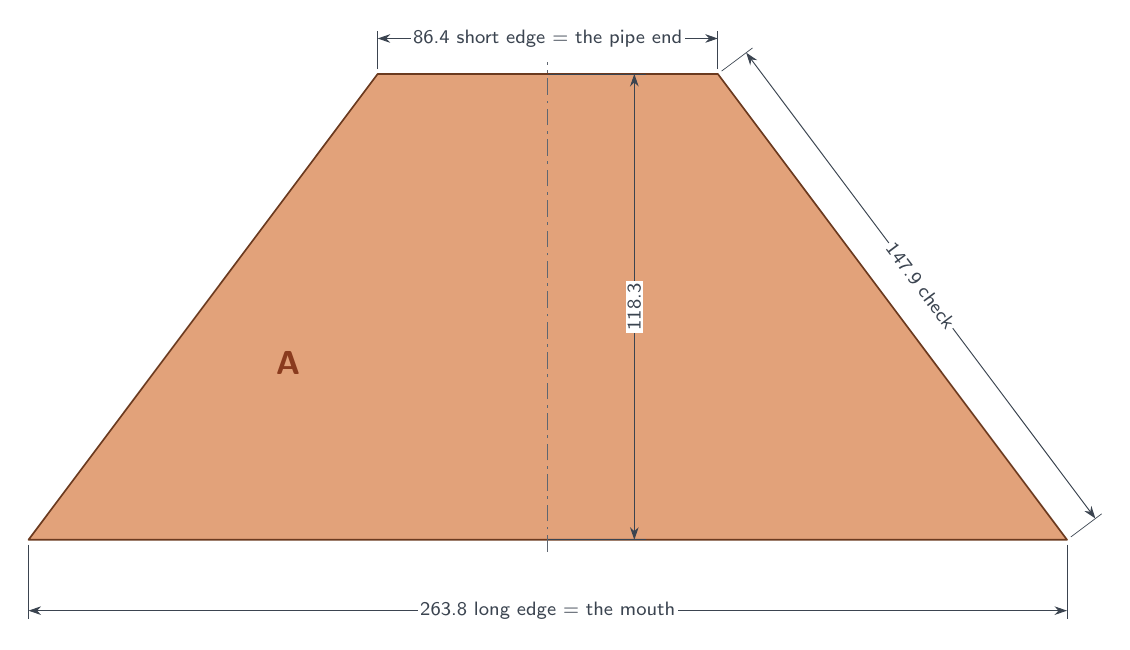
\begin{tikzpicture}[x=0.5mm,y=0.5mm]
\path[wall] (0.00,0.00) -- (263.79,0.00) -- (175.09,118.33) -- (88.69,118.33) -- cycle;
\path[centre] (131.89,-3.00) -- (131.89,121.33);
\path[ext] (0.00,-1.20) -- (0.00,-20.00);
\path[ext] (263.79,-1.20) -- (263.79,-20.00);
\draw[dim] (0.00,-18.00) -- (263.79,-18.00) node[dimlabel]{263.8 long edge = the mouth};
\path[ext] (88.69,119.53) -- (88.69,129.33);
\path[ext] (175.09,119.53) -- (175.09,129.33);
\draw[dim] (88.69,127.33) -- (175.09,127.33) node[dimlabel]{86.4 short edge = the pipe end};
\draw[dim] (153.88,0.00) -- (153.88,118.33) node[dimlabel]{118.3};
\path[ext] (131.89,118.33) -- (156.89,118.33);
\path[ext] (131.89,0.00) -- (156.89,0.00);
\path[ext] (264.75,0.72) -- (272.59,6.60);
\path[ext] (176.05,119.05) -- (183.89,124.92);
\draw[dim] (270.99,5.40) -- (182.29,123.73) node[dimlabel]{147.9 check};
\node[partlabel] at (65.95,44.96) {A};
\end{tikzpicture}

\caption{Piece A, top and bottom flare panel. Cut 2. No tabs: the B tabs lap over its slanted edges.}
\end{figure}
\begin{figure}[H]
\centering
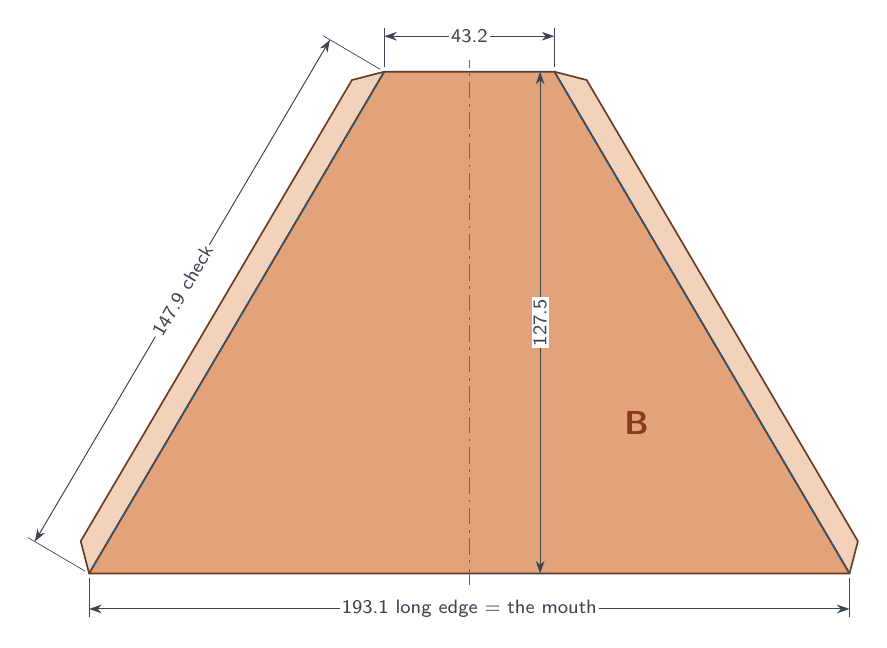
\begin{tikzpicture}[x=0.5mm,y=0.5mm]
\path[tab] (193.14,0.00) -- (118.17,127.47) -- (126.38,125.34) -- (195.27,8.21) -- cycle;
\path[tab] (74.97,127.47) -- (0.00,0.00) -- (-2.13,8.21) -- (66.75,125.34) -- cycle;
\path[wall] (0.00,0.00) -- (193.14,0.00) -- (118.17,127.47) -- (74.97,127.47) -- cycle;
\path[fold] (193.14,0.00) -- (118.17,127.47);
\path[fold] (74.97,127.47) -- (0.00,0.00);
\path[centre] (96.57,-3.00) -- (96.57,130.47);
\path[ext] (0.00,-1.20) -- (0.00,-11.00);
\path[ext] (193.14,-1.20) -- (193.14,-11.00);
\draw[dim] (0.00,-9.00) -- (193.14,-9.00) node[dimlabel]{193.1 long edge = the mouth};
\path[ext] (74.97,128.67) -- (74.97,138.47);
\path[ext] (118.17,128.67) -- (118.17,138.47);
\draw[dim] (74.97,136.47) -- (118.17,136.47) node[dimlabel]{43.2};
\draw[dim] (114.56,0.00) -- (114.56,127.47) node[dimlabel]{127.5};
\path[ext] (96.57,127.47) -- (117.57,127.47);
\path[ext] (96.57,0.00) -- (117.57,0.00);
\path[ext] (-1.03,0.61) -- (-15.52,9.13);
\path[ext] (73.93,128.07) -- (59.45,136.59);
\draw[dim] (-13.79,8.11) -- (61.18,135.58) node[dimlabel]{147.9 check};
\node[partlabel] at (139.06,38.24) {B};
\end{tikzpicture}

\caption{Piece B, side flare panel. Cut 2. The tabs on its slanted edges fold \cornerBend° and wrap over the outside of A.}
\end{figure}

\newpage
\subsection{The pipe pieces, flat}
\begin{figure}[H]
\centering
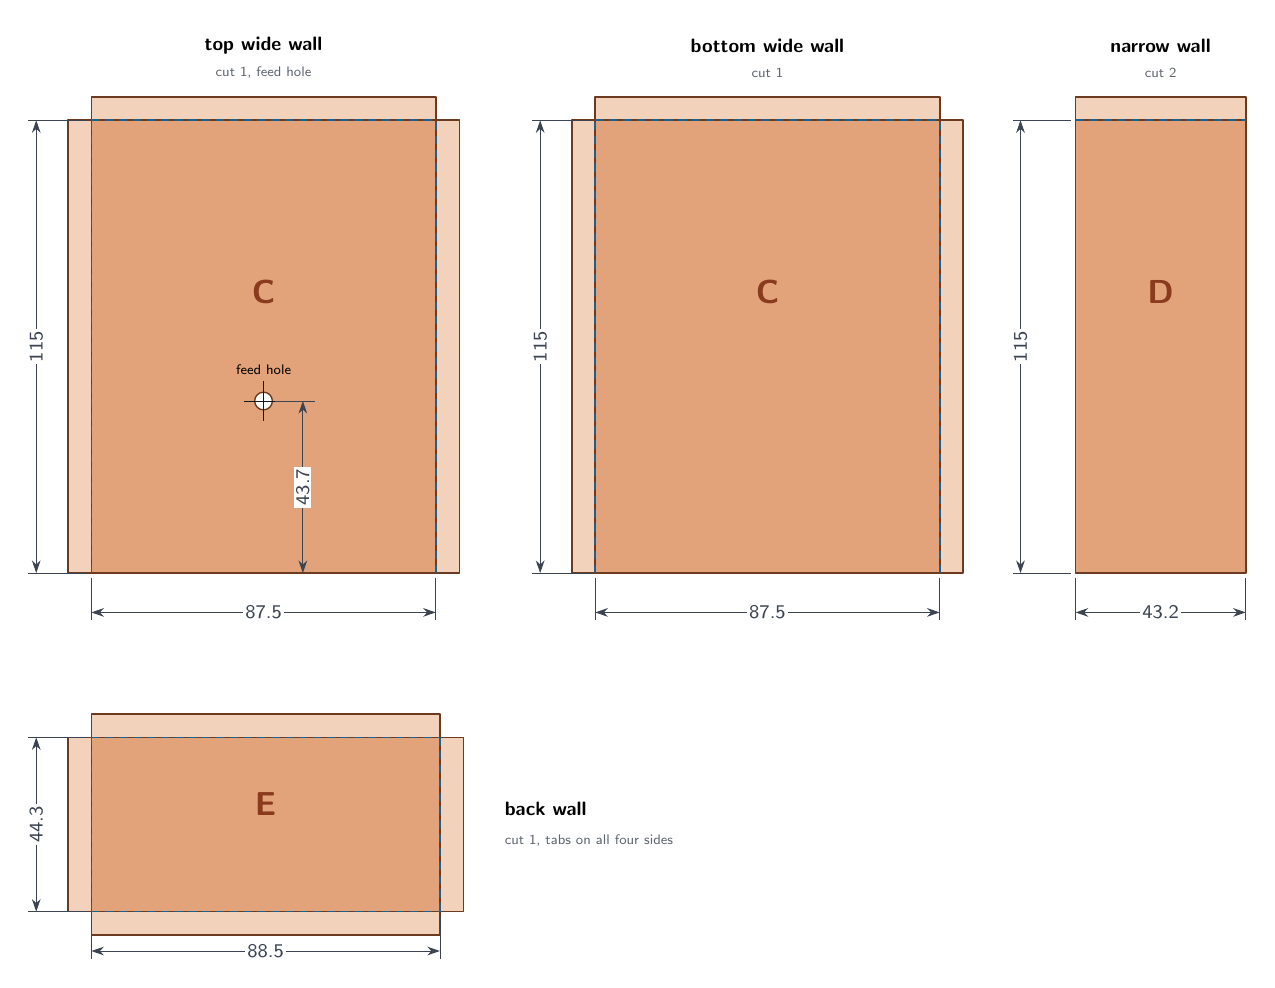
\begin{tikzpicture}[x=0.5mm,y=0.5mm]
\path[tab] (6.00,98.00) -- (12.00,98.00) -- (12.00,213.00) -- (6.00,213.00) -- cycle;
\path[tab] (99.47,98.00) -- (105.47,98.00) -- (105.47,213.00) -- (99.47,213.00) -- cycle;
\path[tab] (12.00,213.00) -- (99.47,213.00) -- (99.47,219.00) -- (12.00,219.00) -- cycle;
\path[wall] (12.00,98.00) -- (99.47,98.00) -- (99.47,213.00) -- (12.00,213.00) -- cycle;
\path[fold] (12.00,98.00) -- (12.00,213.00);
\path[fold] (99.47,98.00) -- (99.47,213.00);
\path[fold] (12.00,213.00) -- (99.47,213.00);
\draw[cuedge,fill=white,line width=0.5pt] (55.73,141.70) circle[radius=2.25];
\path[draw=ink,line width=0.3pt] (50.73,141.70) -- (60.73,141.70);
\path[draw=ink,line width=0.3pt] (55.73,136.70) -- (55.73,146.70);
\node[partlabel] at (55.73,169.30) {C};
\path[ext] (12.00,96.80) -- (12.00,86.00);
\path[ext] (99.47,96.80) -- (99.47,86.00);
\draw[dim] (12.00,88.00) -- (99.47,88.00) node[dimlabel]{87.5};
\path[ext] (10.80,98.00) -- (-4.00,98.00);
\path[ext] (10.80,213.00) -- (-4.00,213.00);
\draw[dim] (-2.00,98.00) -- (-2.00,213.00) node[dimlabel]{115};
\draw[dim] (65.72,98.00) -- (65.72,141.70) node[dimlabel]{43.7};
\path[ext] (58.73,141.70) -- (68.73,141.70);
\node[font=\tiny] at (55.73,149.70) {feed hole};
\node[font=\scriptsize] at (55.73,232.00) {\textbf{top wide wall}};
\node[font=\tiny,text=muted] at (55.73,225.00) {cut 1, feed hole};
\path[tab] (134.00,98.00) -- (140.00,98.00) -- (140.00,213.00) -- (134.00,213.00) -- cycle;
\path[tab] (227.47,98.00) -- (233.47,98.00) -- (233.47,213.00) -- (227.47,213.00) -- cycle;
\path[tab] (140.00,213.00) -- (227.47,213.00) -- (227.47,219.00) -- (140.00,219.00) -- cycle;
\path[wall] (140.00,98.00) -- (227.47,98.00) -- (227.47,213.00) -- (140.00,213.00) -- cycle;
\path[fold] (140.00,98.00) -- (140.00,213.00);
\path[fold] (227.47,98.00) -- (227.47,213.00);
\path[fold] (140.00,213.00) -- (227.47,213.00);
\node[partlabel] at (183.73,169.30) {C};
\path[ext] (140.00,96.80) -- (140.00,86.00);
\path[ext] (227.47,96.80) -- (227.47,86.00);
\draw[dim] (140.00,88.00) -- (227.47,88.00) node[dimlabel]{87.5};
\path[ext] (138.80,98.00) -- (124.00,98.00);
\path[ext] (138.80,213.00) -- (124.00,213.00);
\draw[dim] (126.00,98.00) -- (126.00,213.00) node[dimlabel]{115};
\node[font=\scriptsize] at (183.73,232.00) {\textbf{bottom wide wall}};
\node[font=\tiny,text=muted] at (183.73,225.00) {cut 1};
\path[tab] (262.00,213.00) -- (305.20,213.00) -- (305.20,219.00) -- (262.00,219.00) -- cycle;
\path[wall] (262.00,98.00) -- (305.20,98.00) -- (305.20,213.00) -- (262.00,213.00) -- cycle;
\path[fold] (262.00,213.00) -- (305.20,213.00);
\node[partlabel] at (283.60,169.30) {D};
\path[ext] (262.00,96.80) -- (262.00,86.00);
\path[ext] (305.20,96.80) -- (305.20,86.00);
\draw[dim] (262.00,88.00) -- (305.20,88.00) node[dimlabel]{43.2};
\path[ext] (260.80,98.00) -- (246.00,98.00);
\path[ext] (260.80,213.00) -- (246.00,213.00);
\draw[dim] (248.00,98.00) -- (248.00,213.00) node[dimlabel]{115};
\node[font=\scriptsize] at (283.60,232.00) {\textbf{narrow wall}};
\node[font=\tiny,text=muted] at (283.60,225.00) {cut 2};
\path[tab] (12.00,6.00) -- (100.53,6.00) -- (100.53,12.00) -- (12.00,12.00) -- cycle;
\path[tab] (12.00,56.27) -- (100.53,56.27) -- (100.53,62.27) -- (12.00,62.27) -- cycle;
\path[tab] (6.00,12.00) -- (12.00,12.00) -- (12.00,56.27) -- (6.00,56.27) -- cycle;
\path[tab] (100.53,12.00) -- (106.53,12.00) -- (106.53,56.27) -- (100.53,56.27) -- cycle;
\path[wall] (12.00,12.00) -- (100.53,12.00) -- (100.53,56.27) -- (12.00,56.27) -- cycle;
\path[fold] (12.00,12.00) -- (100.53,12.00);
\path[fold] (12.00,56.27) -- (100.53,56.27);
\path[fold] (12.00,12.00) -- (12.00,56.27);
\path[fold] (100.53,12.00) -- (100.53,56.27);
\node[partlabel] at (56.27,39.44) {E};
\path[ext] (12.00,10.80) -- (12.00,0.00);
\path[ext] (100.53,10.80) -- (100.53,0.00);
\draw[dim] (12.00,2.00) -- (100.53,2.00) node[dimlabel]{88.5};
\path[ext] (10.80,12.00) -- (-4.00,12.00);
\path[ext] (10.80,56.27) -- (-4.00,56.27);
\draw[dim] (-2.00,12.00) -- (-2.00,56.27) node[dimlabel]{44.3};
\node[font=\scriptsize,anchor=west] at (114.53,38.13) {\textbf{back wall}};
\node[font=\tiny,text=muted,anchor=west] at (114.53,30.13) {cut 1, tabs on all four sides};
\end{tikzpicture}

\caption{The pipe pieces at 1\,:\,2, back edge at the bottom. Only one C gets the feed hole: \probeZ\,mm up from the back edge, halfway across. The strips above C and D are the front tabs that become the collar the flare sits on.}
\end{figure}

\subsection{The feed: connector and probe}
\begin{figure}[H]
\centering
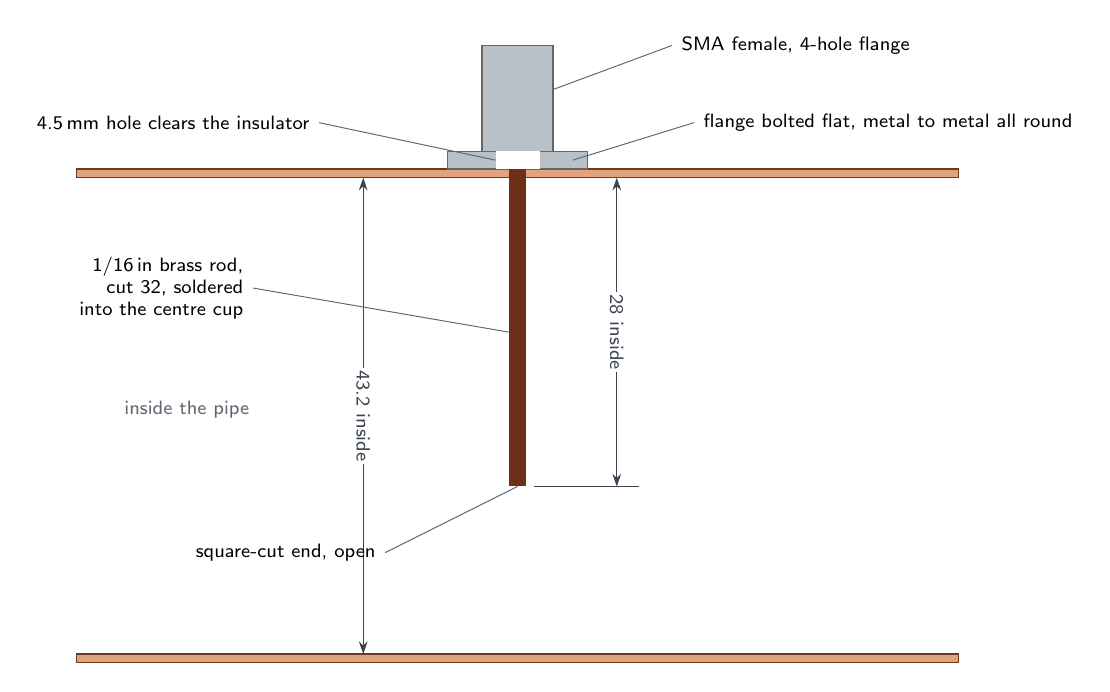
\begin{tikzpicture}[x=1.4mm,y=1.4mm,font=\scriptsize]
  % wall cross-section
  \fill[cuout] (-40,0) rectangle (40,0.8);
  \draw[cuedge] (-40,0) rectangle (40,0.8);
  \fill[cuout] (-40,-43.2) rectangle (40,-44);
  \draw[cuedge] (-40,-43.2) rectangle (40,-44);
  \node[text=muted] at (-30,-21) {inside the pipe};
  % flange
  \path[alupart] (-6.35,0.8) rectangle (6.35,2.4);
  \path[alupart] (-3.2,2.4) rectangle (3.2,12);
  \fill[white] (-2,0.8) rectangle (2,2.4);
  % probe
  \fill[accent!80!black] (-0.8,0.8) rectangle (0.8,-28);
  \draw[dim] (9,0) -- (9,-28) node[dimlabel]{\probeLen\ inside};
  \draw[ext] (1.5,-28) -- (11,-28);
  \draw[dim] (-14,0) -- (-14,-43.2) node[dimlabel]{\pipeH\ inside};
  \draw[callout] (3.2,8) -- (14,12) node[right]{SMA female, 4-hole flange};
  \draw[callout] (5,1.6) -- (16,5) node[right]{flange bolted flat, metal to metal all round};
  \draw[callout] (-0.8,-14) -- (-24,-10) node[left,align=right]{1/16\,in brass rod,\\cut \rodCut, soldered\\into the centre cup};
  \draw[callout] (0,-28) -- (-12,-34) node[left]{square-cut end, open};
  \draw[callout] (-2,1.6) -- (-18,5) node[left]{4.5\,mm hole clears the insulator};
\end{tikzpicture}
\caption{Section through the top wide wall at the feed, full height of the pipe shown. The flange's four 2.7\,mm holes take M2.5 or 2-56 screws (M3 is too big).}
\end{figure}

\newpage
\subsection{One horn per sheet}\label{sec:sheet}
Everything for one horn fits on one 12\,×\,24\,in sheet with a 3\,mm cutting gap between pieces and 4\,mm clear of the edge. Each horn uses about \sheetIn\ square inches, \sheetPct\,\% of a sheet. Two sheets do \emph{not} make three horns: what is left over is too narrow for another set of flare panels. \textbf{Three horns need three sheets}; a fourth is cheap insurance against a mis-cut.

\begin{figure}[H]
\centering
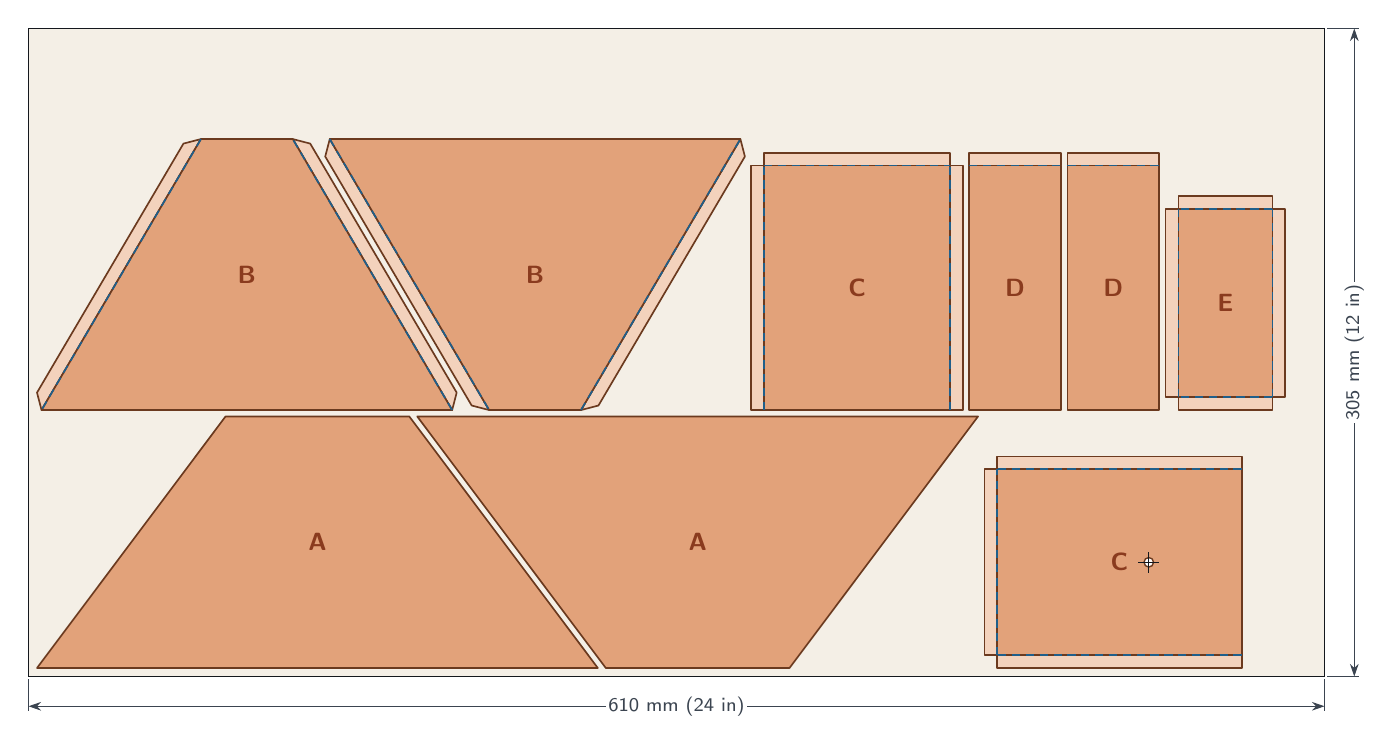
\begin{tikzpicture}[x=0.27mm,y=0.27mm]
\path[draw=ink,line width=0.6pt,fill=boxbg] (0,0) rectangle (609.60,304.80);
\path[wall] (4.00,4.00) -- (267.79,4.00) -- (179.09,122.33) -- (92.69,122.33) -- cycle;
\node[font=\bfseries\small,text=accent] at (135.89,63.16) {A};
\path[wall] (446.63,122.33) -- (182.84,122.33) -- (271.54,4.00) -- (357.94,4.00) -- cycle;
\node[font=\bfseries\small,text=accent] at (314.74,63.16) {A};
\path[tab] (570.63,4.00) -- (570.63,10.00) -- (455.63,10.00) -- (455.63,4.00) -- cycle;
\path[tab] (570.63,97.47) -- (570.63,103.47) -- (455.63,103.47) -- (455.63,97.47) -- cycle;
\path[tab] (455.63,10.00) -- (455.63,97.47) -- (449.63,97.47) -- (449.63,10.00) -- cycle;
\path[wall] (570.63,10.00) -- (570.63,97.47) -- (455.63,97.47) -- (455.63,10.00) -- cycle;
\path[fold] (570.63,10.00) -- (455.63,10.00);
\path[fold] (570.63,97.47) -- (455.63,97.47);
\path[fold] (455.63,10.00) -- (455.63,97.47);
\draw[cuedge,fill=white,line width=0.5pt] (526.93,53.73) circle[radius=2.25];
\path[draw=ink,line width=0.3pt] (521.93,53.73) -- (531.93,53.73);
\path[draw=ink,line width=0.3pt] (526.93,48.73) -- (526.93,58.73);
\node[font=\bfseries\small,text=accent] at (513.13,53.73) {C};
\path[tab] (199.27,125.33) -- (124.30,252.79) -- (132.51,250.66) -- (201.40,133.54) -- cycle;
\path[tab] (81.10,252.79) -- (6.13,125.33) -- (4.00,133.54) -- (72.88,250.66) -- cycle;
\path[wall] (6.13,125.33) -- (199.27,125.33) -- (124.30,252.79) -- (81.10,252.79) -- cycle;
\path[fold] (199.27,125.33) -- (124.30,252.79);
\path[fold] (81.10,252.79) -- (6.13,125.33);
\node[font=\bfseries\small,text=accent] at (102.70,189.06) {B};
\path[tab] (141.70,252.79) -- (216.67,125.33) -- (208.45,127.46) -- (139.57,244.58) -- cycle;
\path[tab] (259.87,125.33) -- (334.84,252.79) -- (336.97,244.58) -- (268.08,127.46) -- cycle;
\path[wall] (334.84,252.79) -- (141.70,252.79) -- (216.67,125.33) -- (259.87,125.33) -- cycle;
\path[fold] (141.70,252.79) -- (216.67,125.33);
\path[fold] (259.87,125.33) -- (334.84,252.79);
\node[font=\bfseries\small,text=accent] at (238.27,189.06) {B};
\path[tab] (339.97,125.33) -- (345.97,125.33) -- (345.97,240.33) -- (339.97,240.33) -- cycle;
\path[tab] (433.43,125.33) -- (439.43,125.33) -- (439.43,240.33) -- (433.43,240.33) -- cycle;
\path[tab] (345.97,240.33) -- (433.43,240.33) -- (433.43,246.33) -- (345.97,246.33) -- cycle;
\path[wall] (345.97,125.33) -- (433.43,125.33) -- (433.43,240.33) -- (345.97,240.33) -- cycle;
\path[fold] (345.97,125.33) -- (345.97,240.33);
\path[fold] (433.43,125.33) -- (433.43,240.33);
\path[fold] (345.97,240.33) -- (433.43,240.33);
\node[font=\bfseries\small,text=accent] at (389.70,182.83) {C};
\path[tab] (442.43,240.33) -- (485.63,240.33) -- (485.63,246.33) -- (442.43,246.33) -- cycle;
\path[wall] (442.43,125.33) -- (485.63,125.33) -- (485.63,240.33) -- (442.43,240.33) -- cycle;
\path[fold] (442.43,240.33) -- (485.63,240.33);
\node[font=\bfseries\small,text=accent] at (464.03,182.83) {D};
\path[tab] (488.63,240.33) -- (531.83,240.33) -- (531.83,246.33) -- (488.63,246.33) -- cycle;
\path[wall] (488.63,125.33) -- (531.83,125.33) -- (531.83,240.33) -- (488.63,240.33) -- cycle;
\path[fold] (488.63,240.33) -- (531.83,240.33);
\node[font=\bfseries\small,text=accent] at (510.23,182.83) {D};
\path[tab] (591.10,131.33) -- (591.10,219.86) -- (585.10,219.86) -- (585.10,131.33) -- cycle;
\path[tab] (540.83,131.33) -- (540.83,219.86) -- (534.83,219.86) -- (534.83,131.33) -- cycle;
\path[tab] (585.10,125.33) -- (585.10,131.33) -- (540.83,131.33) -- (540.83,125.33) -- cycle;
\path[tab] (585.10,219.86) -- (585.10,225.86) -- (540.83,225.86) -- (540.83,219.86) -- cycle;
\path[wall] (585.10,131.33) -- (585.10,219.86) -- (540.83,219.86) -- (540.83,131.33) -- cycle;
\path[fold] (585.10,131.33) -- (585.10,219.86);
\path[fold] (540.83,131.33) -- (540.83,219.86);
\path[fold] (585.10,131.33) -- (540.83,131.33);
\path[fold] (585.10,219.86) -- (540.83,219.86);
\node[font=\bfseries\small,text=accent] at (562.97,175.59) {E};
\path[ext] (0.00,-1.20) -- (0.00,-16.00);
\path[ext] (609.60,-1.20) -- (609.60,-16.00);
\draw[dim] (0.00,-14.00) -- (609.60,-14.00) node[dimlabel]{610 mm (24 in)};
\path[ext] (610.80,0.00) -- (625.60,0.00);
\path[ext] (610.80,304.80) -- (625.60,304.80);
\draw[dim] (623.60,0.00) -- (623.60,304.80) node[dimlabel]{305 mm (12 in)};
\end{tikzpicture}

\caption{One horn's nine pieces on one sheet, to scale. Turn every second trapezoid round so the pair nest. The spare strip along the top is for practising a fold and a soldered seam first.}
\end{figure}

\subsubsection*{Marking a trapezoid accurately}
Never mark the slanted edges by measuring along them. Draw the two parallel edges and a centre line square to them, measure half the width out each side of the centre line on each parallel, then join the points. The slant comes out right by itself; check it with the rule against \seam. The full-size templates on the next pages are half-templates for exactly this reason: trace one side, flip the template over on the centre line, trace the other.

\begin{note}[Using the full-size templates]
Print pages \pageref{tmpl:A}–\pageref{tmpl:pipe} at \textbf{100\,\% / actual size}. Measure the 50\,mm square on each page; if it is not 50.0\,mm, your printer scaled it and the cut will be wrong. Cut the paper out, tape it to the copper with the outside face up, and scribe round it. The numbers on the drawing win over the paper if they disagree.
\end{note}

% ── 1:1 templates
\newpage
\subsection{Template: flare panel A (full size)}\label{tmpl:A}
\begin{center}
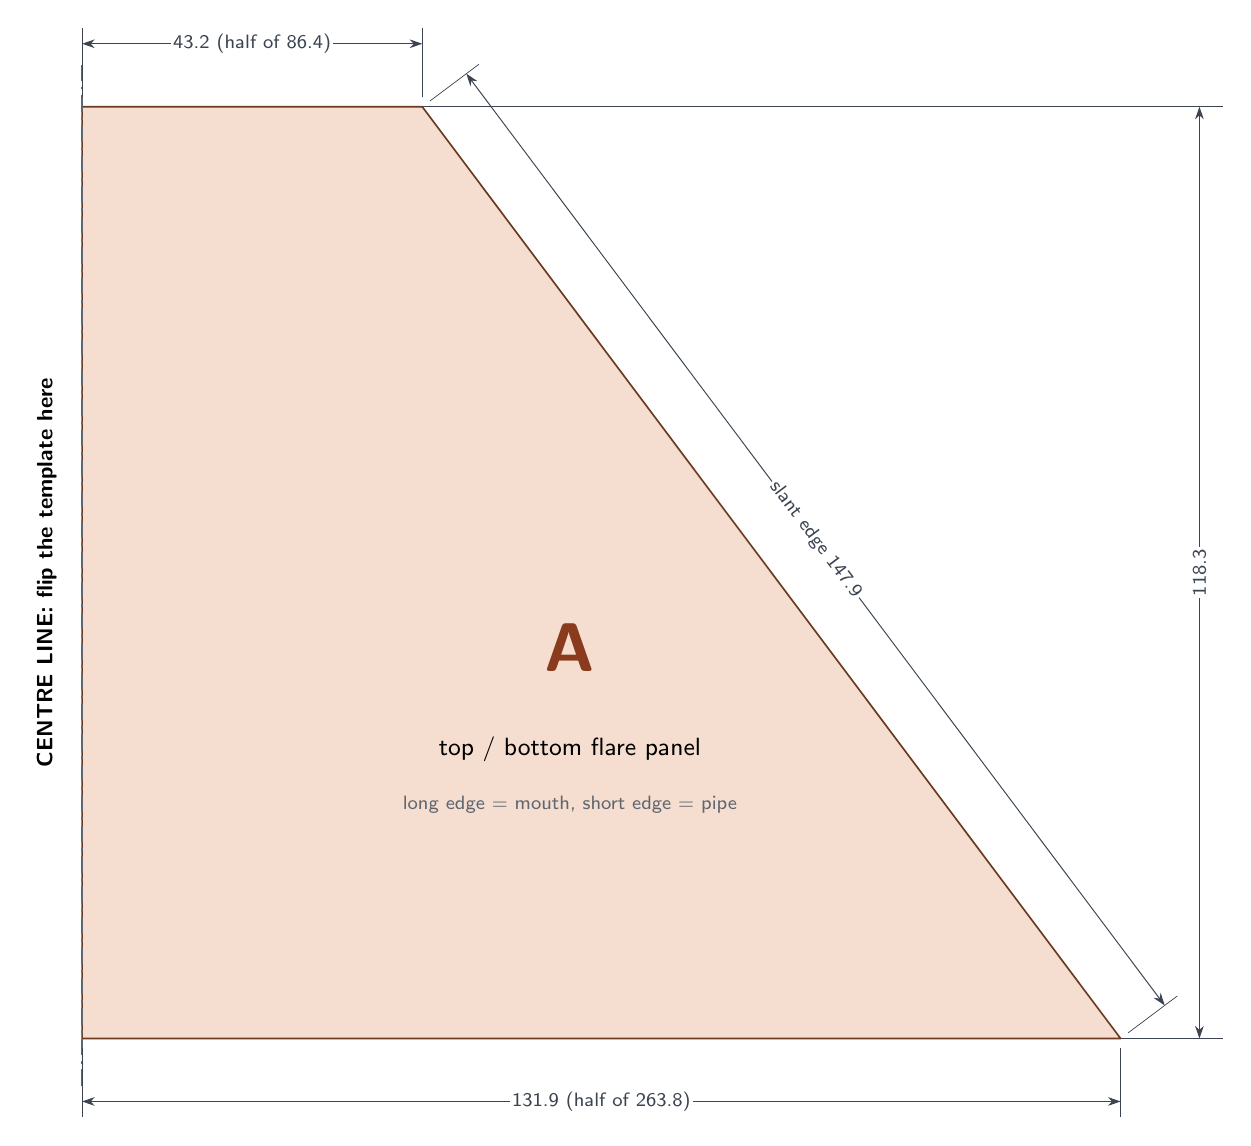
\begin{tikzpicture}[x=1.0mm,y=1.0mm]
\path[wall,fill=cuout!35] (0.00,0.00) -- (131.89,0.00) -- (43.20,118.33) -- (0.00,118.33) -- cycle;
\path[centre,line width=0.6pt] (0.00,-6.00) -- (0.00,124.33);
\node[rotate=90,font=\footnotesize\bfseries,anchor=south] at (-2.00,59.16) {CENTRE LINE: flip the template here};
\path[ext] (0.00,-1.20) -- (0.00,-10.00);
\path[ext] (131.89,-1.20) -- (131.89,-10.00);
\draw[dim] (0.00,-8.00) -- (131.89,-8.00) node[dimlabel]{131.9 (half of 263.8)};
\path[ext] (0.00,119.53) -- (0.00,128.33);
\path[ext] (43.20,119.53) -- (43.20,128.33);
\draw[dim] (0.00,126.33) -- (43.20,126.33) node[dimlabel]{43.2 (half of 86.4)};
\draw[dim] (141.90,0.00) -- (141.90,118.33) node[dimlabel]{118.3};
\path[ext] (43.20,118.33) -- (144.89,118.33);
\path[ext] (131.89,0.00) -- (144.89,0.00);
\path[ext] (132.85,0.72) -- (139.09,5.40);
\path[ext] (44.16,119.05) -- (50.40,123.73);
\draw[dim] (137.49,4.20) -- (48.80,122.53) node[dimlabel]{slant edge 147.9};
\node[font=\Huge\bfseries,text=accent] at (61.95,49.70) {A};
\node[font=\small] at (61.95,36.70) {top / bottom flare panel};
\node[font=\scriptsize,text=muted] at (61.95,29.70) {long edge = mouth, short edge = pipe};
\end{tikzpicture}

\end{center}
\vfill
\begin{center}\checksquare\end{center}

\newpage
\subsection{Template: flare panel B (full size)}\label{tmpl:B}
\begin{center}
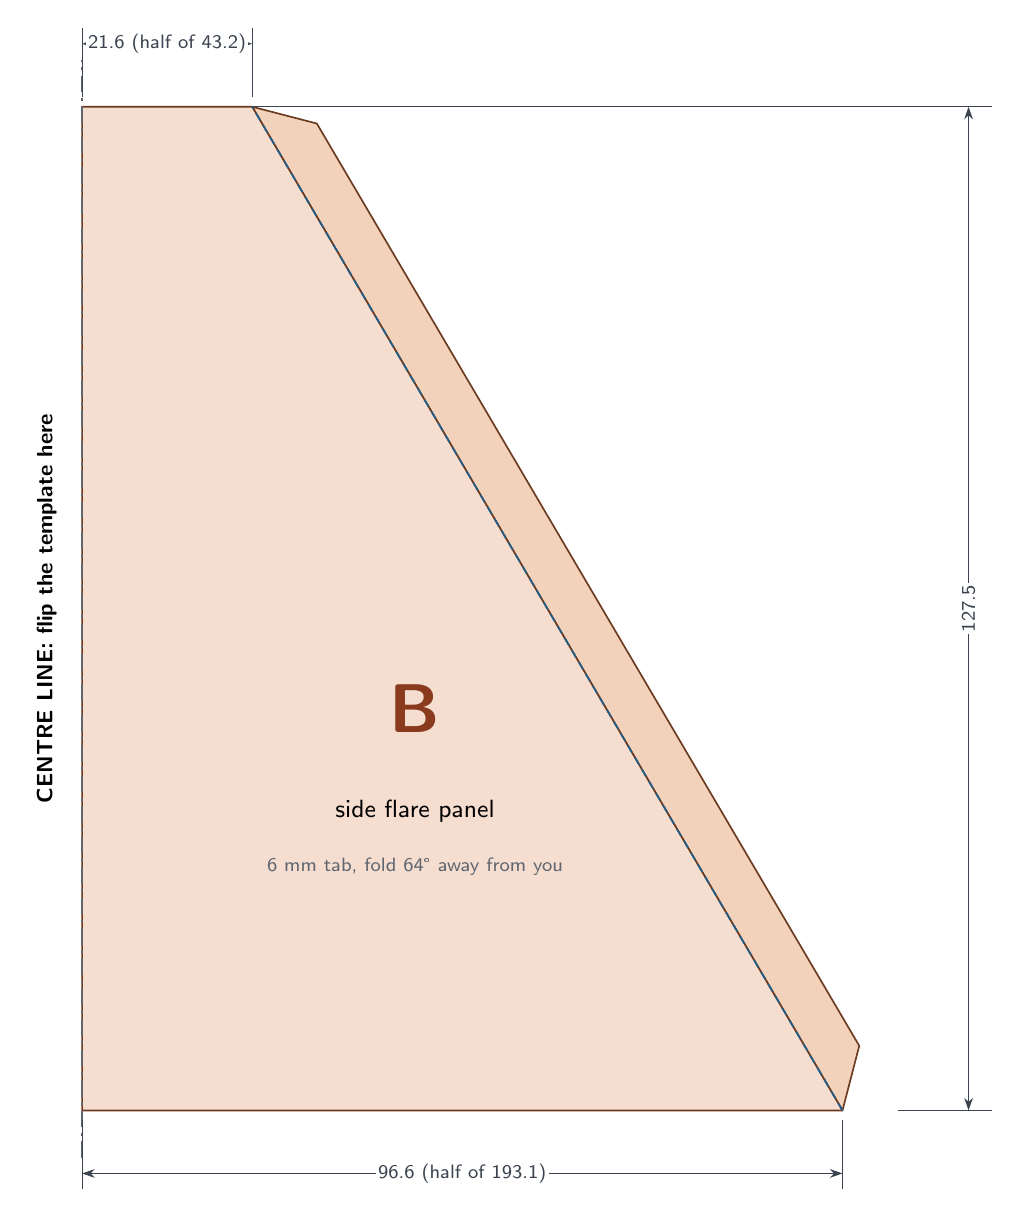
\begin{tikzpicture}[x=1.0mm,y=1.0mm]
\path[tab] (96.57,0.00) -- (21.60,127.47) -- (29.81,125.34) -- (98.70,8.21) -- cycle;
\path[wall,fill=cuout!35] (0.00,0.00) -- (96.57,0.00) -- (21.60,127.47) -- (0.00,127.47) -- cycle;
\path[fold] (96.57,0.00) -- (21.60,127.47);
\path[centre,line width=0.6pt] (0.00,-6.00) -- (0.00,133.47);
\node[rotate=90,font=\footnotesize\bfseries,anchor=south] at (-2.00,63.73) {CENTRE LINE: flip the template here};
\path[ext] (0.00,-1.20) -- (0.00,-10.00);
\path[ext] (96.57,-1.20) -- (96.57,-10.00);
\draw[dim] (0.00,-8.00) -- (96.57,-8.00) node[dimlabel]{96.6 (half of 193.1)};
\path[ext] (0.00,128.67) -- (0.00,137.47);
\path[ext] (21.60,128.67) -- (21.60,137.47);
\draw[dim] (0.00,135.47) -- (21.60,135.47) node[dimlabel]{21.6 (half of 43.2)};
\draw[dim] (112.58,0.00) -- (112.58,127.47) node[dimlabel]{127.5};
\path[ext] (21.60,127.47) -- (115.57,127.47);
\path[ext] (103.57,0.00) -- (115.57,0.00);
\node[font=\Huge\bfseries,text=accent] at (42.28,50.99) {B};
\node[font=\small] at (42.28,37.99) {side flare panel};
\node[font=\scriptsize,text=muted] at (42.28,30.99) {6 mm tab, fold 64° away from you};
\end{tikzpicture}

\end{center}
\vfill
\begin{center}\checksquare\end{center}

\newpage
\subsection{Template: the pipe, C, D and E (full size)}\label{tmpl:pipe}
\begin{center}
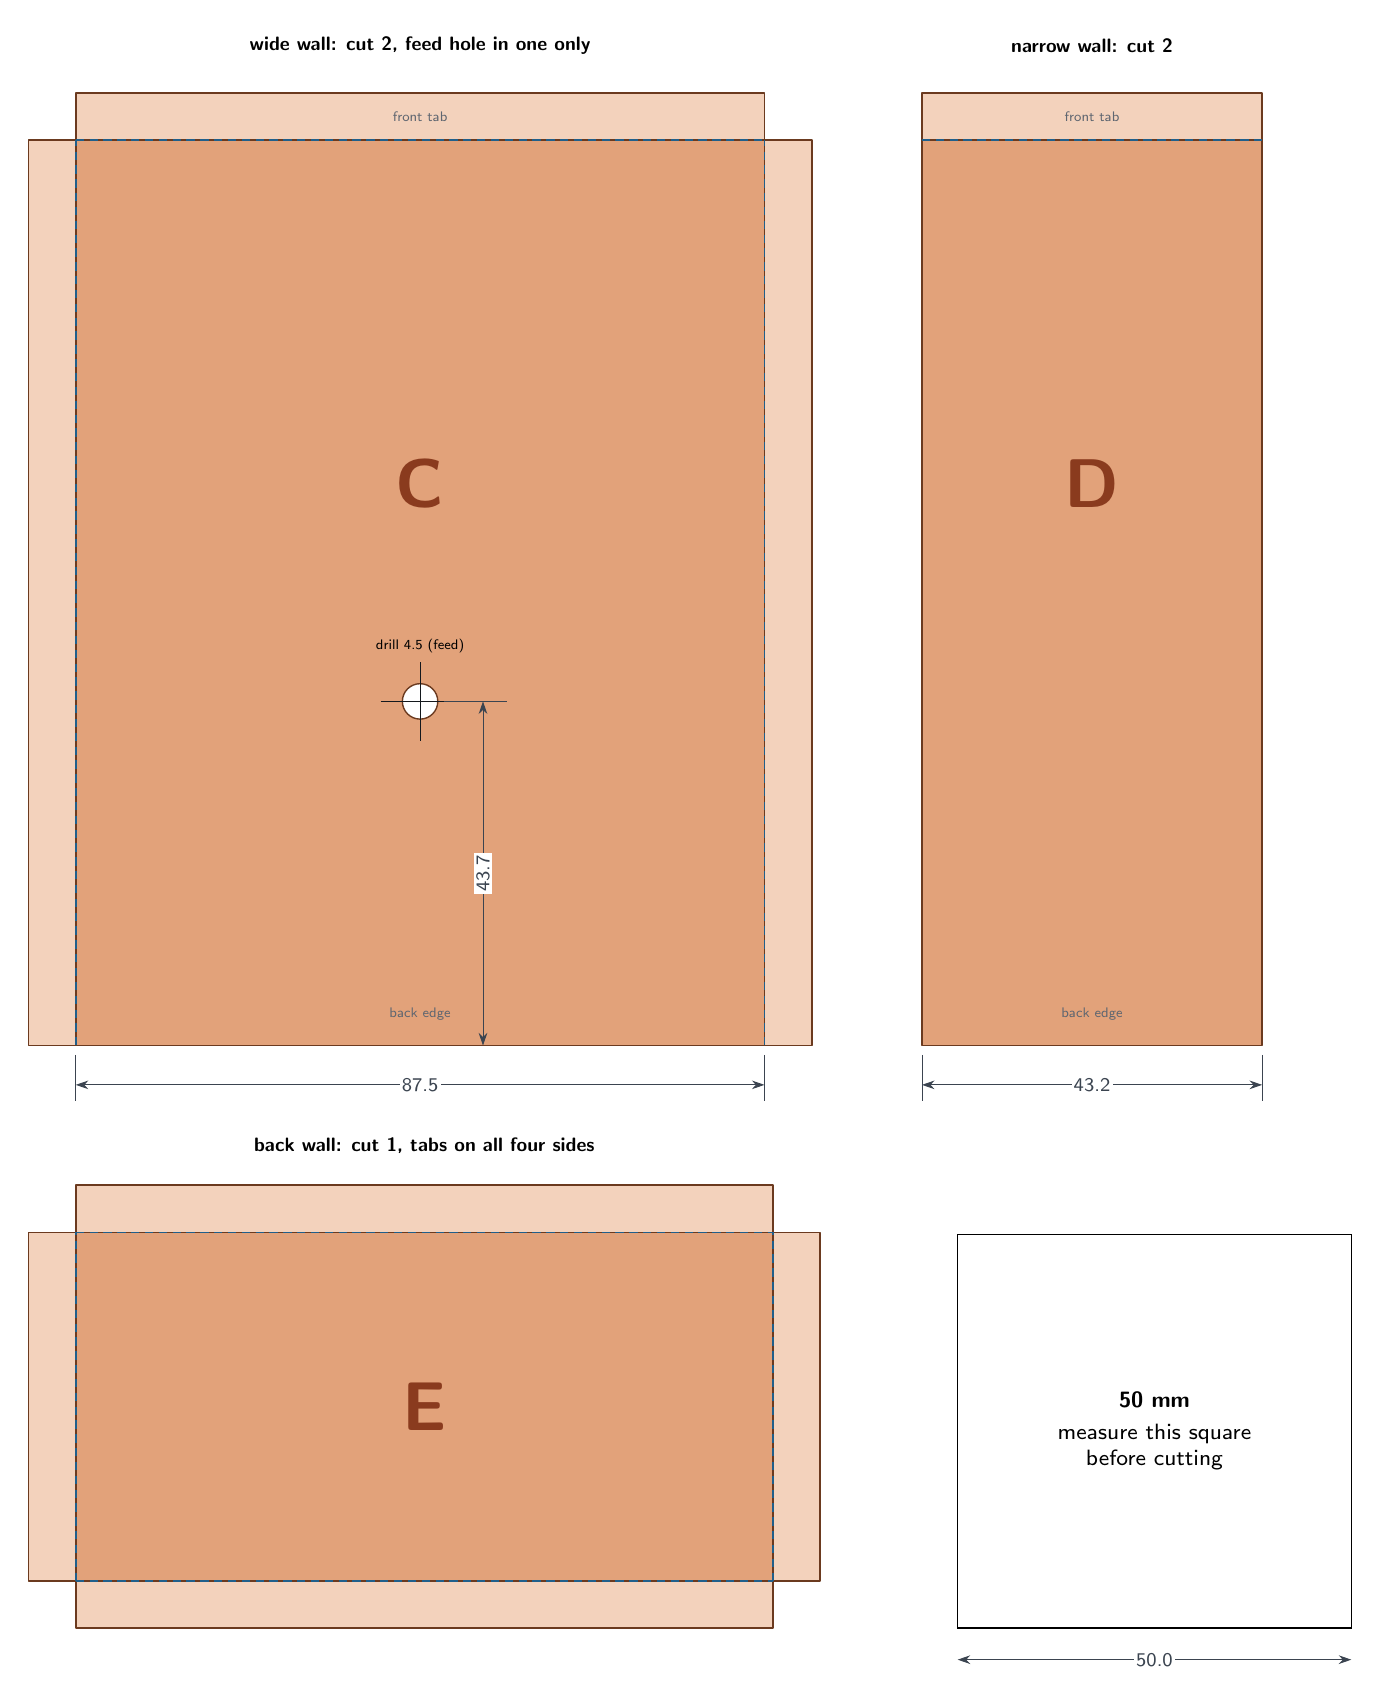
\begin{tikzpicture}[x=1.0mm,y=1.0mm]
\path[tab] (0.00,82.00) -- (6.00,82.00) -- (6.00,197.00) -- (0.00,197.00) -- cycle;
\path[tab] (93.47,82.00) -- (99.47,82.00) -- (99.47,197.00) -- (93.47,197.00) -- cycle;
\path[tab] (6.00,197.00) -- (93.47,197.00) -- (93.47,203.00) -- (6.00,203.00) -- cycle;
\path[wall] (6.00,82.00) -- (93.47,82.00) -- (93.47,197.00) -- (6.00,197.00) -- cycle;
\path[fold] (6.00,82.00) -- (6.00,197.00);
\path[fold] (93.47,82.00) -- (93.47,197.00);
\path[fold] (6.00,197.00) -- (93.47,197.00);
\draw[cuedge,fill=white,line width=0.5pt] (49.73,125.70) circle[radius=2.25];
\path[draw=ink,line width=0.3pt] (44.73,125.70) -- (54.73,125.70);
\path[draw=ink,line width=0.3pt] (49.73,120.70) -- (49.73,130.70);
\node[font=\Huge\bfseries,text=accent] at (49.73,153.30) {C};
\node[font=\scriptsize\bfseries] at (49.73,209.00) {wide wall: cut 2, feed hole in one only};
\node[font=\tiny,text=muted] at (49.73,86.00) {back edge};
\node[font=\tiny,text=muted] at (49.73,200.00) {front tab};
\path[ext] (6.00,80.80) -- (6.00,75.00);
\path[ext] (93.47,80.80) -- (93.47,75.00);
\draw[dim] (6.00,77.00) -- (93.47,77.00) node[dimlabel]{87.5};
\draw[dim] (57.72,82.00) -- (57.72,125.70) node[dimlabel]{43.7};
\path[ext] (52.73,125.70) -- (60.73,125.70);
\node[font=\tiny] at (49.73,132.70) {drill 4.5 (feed)};
\path[tab] (113.47,197.00) -- (156.67,197.00) -- (156.67,203.00) -- (113.47,203.00) -- cycle;
\path[wall] (113.47,82.00) -- (156.67,82.00) -- (156.67,197.00) -- (113.47,197.00) -- cycle;
\path[fold] (113.47,197.00) -- (156.67,197.00);
\node[font=\Huge\bfseries,text=accent] at (135.07,153.30) {D};
\node[font=\scriptsize\bfseries] at (135.07,209.00) {narrow wall: cut 2};
\node[font=\tiny,text=muted] at (135.07,86.00) {back edge};
\node[font=\tiny,text=muted] at (135.07,200.00) {front tab};
\path[ext] (113.47,80.80) -- (113.47,75.00);
\path[ext] (156.67,80.80) -- (156.67,75.00);
\draw[dim] (113.47,77.00) -- (156.67,77.00) node[dimlabel]{43.2};
\path[tab] (6.00,8.00) -- (94.53,8.00) -- (94.53,14.00) -- (6.00,14.00) -- cycle;
\path[tab] (6.00,58.27) -- (94.53,58.27) -- (94.53,64.27) -- (6.00,64.27) -- cycle;
\path[tab] (0.00,14.00) -- (6.00,14.00) -- (6.00,58.27) -- (0.00,58.27) -- cycle;
\path[tab] (94.53,14.00) -- (100.53,14.00) -- (100.53,58.27) -- (94.53,58.27) -- cycle;
\path[wall] (6.00,14.00) -- (94.53,14.00) -- (94.53,58.27) -- (6.00,58.27) -- cycle;
\path[fold] (6.00,14.00) -- (94.53,14.00);
\path[fold] (6.00,58.27) -- (94.53,58.27);
\path[fold] (6.00,14.00) -- (6.00,58.27);
\path[fold] (94.53,14.00) -- (94.53,58.27);
\node[font=\Huge\bfseries,text=accent] at (50.27,36.13) {E};
\node[font=\scriptsize\bfseries] at (50.27,69.27) {back wall: cut 1, tabs on all four sides};
\draw[line width=0.5pt] (118.00,8.00) rectangle (168.00,58.00);
\node[font=\footnotesize,align=center] at (143.00,33.00) {\textbf{50 mm}\\[2pt]measure this square\\before cutting};
\draw[dim] (118.00,4.00) -- (168.00,4.00) node[dimlabel]{50.0};
\end{tikzpicture}

\end{center}

\newpage
% ───────────────────────────────────────────────────────────── 4 the frame
\section{The frame}\label{sec:frame}

A plywood board, two square uprights, two cross beams and two diagonal braces. Wood is easiest; aluminium bar of the same section works the same way. Horns are \emph{rolled} 90° on their side: the pipe's wide walls face left and right and the long side of the mouth runs up and down. Roll all three the same way, so every connector points to the left as you sit behind the bench. (Left and right in this document are always as seen from there, the operator's seat, with the horns pointing away from you into the room.) That is what the beam heights below assume, and it makes the two receive cables follow the same path when the second receiver goes in.

\begin{figure}[H]
\centering
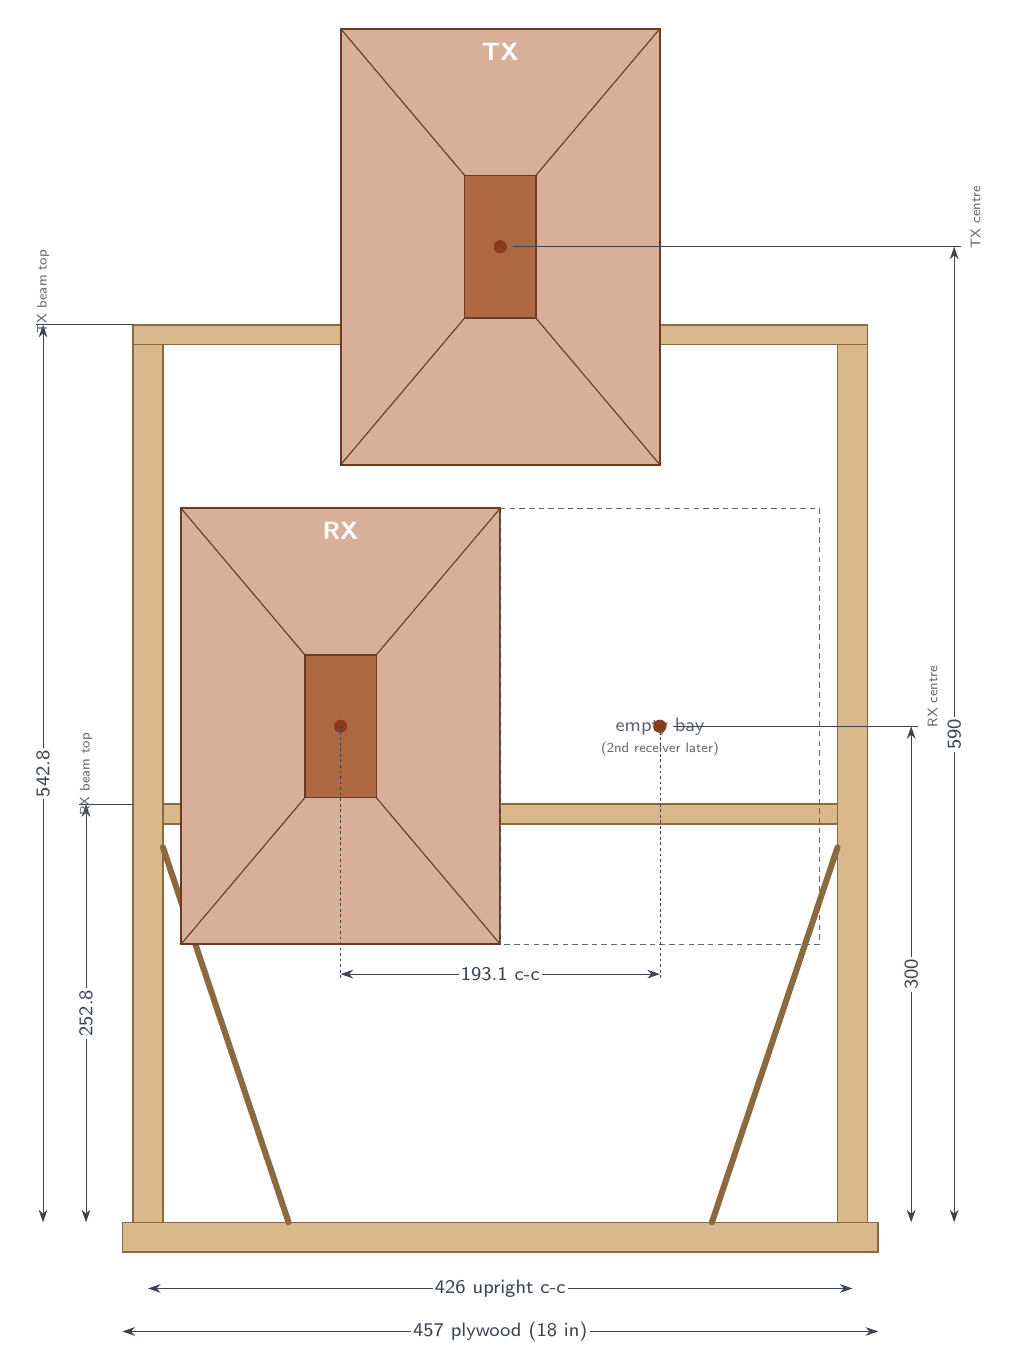
\begin{tikzpicture}[x=0.21mm,y=0.21mm]
\path[woodpart] (-228.50,-18.00) rectangle (228.50,0.00);
\path[woodpart] (-222.00,0.00) rectangle (-204.00,530.80);
\path[draw=woodedge,line width=2.2pt,line cap=round] (-204.00,226.80) -- (-128.00,0.00);
\path[woodpart] (204.00,0.00) rectangle (222.00,530.80);
\path[draw=woodedge,line width=2.2pt,line cap=round] (204.00,226.80) -- (128.00,0.00);
\path[woodpart] (-204.00,240.80) rectangle (204.00,252.80);
\path[woodpart] (-222.00,530.80) rectangle (222.00,542.80);
\path[draw=cuedge,line width=0.7pt,fill=cuin!55] (-193.12,168.11) rectangle (0.02,431.89);
\path[draw=cuedge,line width=0.5pt,fill=cuin!95!black] (-118.15,256.80) rectangle (-74.95,343.20);
\path[draw=cuedge,line width=0.4pt] (-74.95,343.20) -- (0.02,431.89);
\path[draw=cuedge,line width=0.4pt] (-74.95,256.80) -- (0.02,168.11);
\path[draw=cuedge,line width=0.4pt] (-118.15,343.20) -- (-193.12,431.89);
\path[draw=cuedge,line width=0.4pt] (-118.15,256.80) -- (-193.12,168.11);
\node[font=\bfseries\small,text=white] at (-96.55,417.89) {RX};
\fill[accent] (-96.55,300.00) circle[radius=4];
\path[hidden] (-0.02,168.11) rectangle (193.12,431.89);
\node[font=\scriptsize,text=muted,align=center] at (96.55,300.00) {empty bay};
\node[font=\tiny,text=muted] at (96.55,286.00) {(2nd receiver later)};
\fill[accent] (96.55,300.00) circle[radius=4];
\path[draw=cuedge,line width=0.7pt,fill=cuin!55] (-96.57,458.11) rectangle (96.57,721.89);
\path[draw=cuedge,line width=0.5pt,fill=cuin!95!black] (-21.60,546.80) rectangle (21.60,633.20);
\path[draw=cuedge,line width=0.4pt] (21.60,633.20) -- (96.57,721.89);
\path[draw=cuedge,line width=0.4pt] (21.60,546.80) -- (96.57,458.11);
\path[draw=cuedge,line width=0.4pt] (-21.60,633.20) -- (-96.57,721.89);
\path[draw=cuedge,line width=0.4pt] (-21.60,546.80) -- (-96.57,458.11);
\node[font=\bfseries\small,text=white] at (0.00,707.89) {TX};
\fill[accent] (0.00,590.00) circle[radius=4];
\draw[dim] (-96.55,150.12) -- (96.55,150.12) node[dimlabel]{193.1 c-c};
\path[ext,dash pattern=on 1pt off 1pt] (-96.55,300.00) -- (-96.55,146.11);
\path[ext,dash pattern=on 1pt off 1pt] (96.55,300.00) -- (96.55,146.11);
\draw[dim] (248.51,0.00) -- (248.51,300.00) node[dimlabel]{300};
\draw[dim] (274.51,0.00) -- (274.51,590.00) node[dimlabel]{590};
\path[ext] (104.55,300.00) -- (252.50,300.00);
\path[ext] (8.00,590.00) -- (278.50,590.00);
\draw[dim] (-250.51,0.00) -- (-250.51,252.80) node[dimlabel]{252.8};
\draw[dim] (-276.51,0.00) -- (-276.51,542.80) node[dimlabel]{542.8};
\path[ext] (-222.00,252.80) -- (-254.50,252.80);
\path[ext] (-222.00,542.80) -- (-280.50,542.80);
\draw[dim] (-213.00,-39.99) -- (213.00,-39.99) node[dimlabel]{426 upright c-c};
\draw[dim] (-228.50,-65.99) -- (228.50,-65.99) node[dimlabel]{457 plywood (18 in)};
\node[font=\tiny,text=muted,rotate=90] at (261.50,318.00) {RX centre};
\node[font=\tiny,text=muted,rotate=90] at (287.50,608.00) {TX centre};
\node[font=\tiny,text=muted,rotate=90] at (-250.50,270.80) {RX beam top};
\node[font=\tiny,text=muted,rotate=90] at (-276.50,562.80) {TX beam top};
\end{tikzpicture}

\caption{The frame from behind, from where you sit, 1\,:\,4; the horns point away from you. The receive horn and the empty bay sit side by side on the lower beam, mouths touching; the transmit horn sits centred on the top beam, \rowGap\,mm clear of them. Red dots are the horn centre lines. Braces run from the uprights down to the board \braceFootX\,mm either side of centre.}
\end{figure}

\newpage
\begin{figure}[H]
\centering
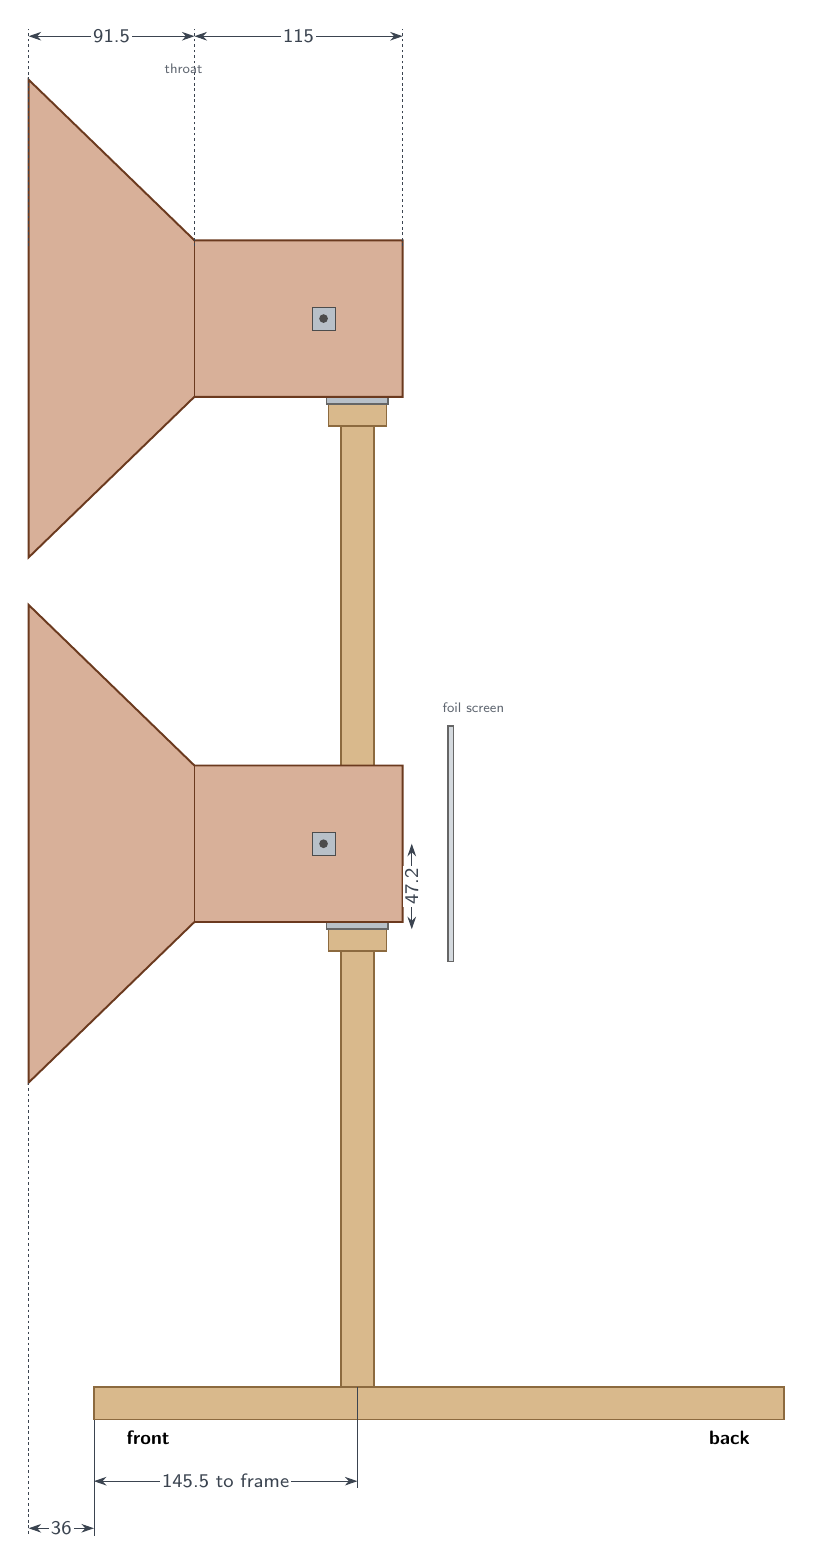
\begin{tikzpicture}[x=0.23mm,y=0.23mm]
\path[woodpart] (-190.50,-18.00) rectangle (190.50,0.00);
\path[woodpart] (-54.00,0.00) rectangle (-36.00,530.80);
\path[woodpart] (-61.00,240.80) rectangle (-29.00,252.80);
\path[woodpart] (-61.00,530.80) rectangle (-29.00,542.80);
\path[alupart] (-62.00,252.80) rectangle (-28.00,284.80);
\path[draw=cuedge,line width=0.7pt,fill=cuin!55] (-226.55,168.11) -- (-135.00,256.80) -- (-20.00,256.80) -- (-20.00,343.20) -- (-135.00,343.20) -- (-226.55,431.89) -- cycle;
\path[draw=cuedge,line width=0.4pt] (-135.00,256.80) -- (-135.00,343.20);
\path[draw=black!70,fill=alu,line width=0.4pt] (-70.05,293.65) rectangle (-57.35,306.35);
\fill[black!70] (-63.70,300.00) circle[radius=2.4];
\path[alupart] (-62.00,542.80) rectangle (-28.00,574.80);
\path[draw=cuedge,line width=0.7pt,fill=cuin!55] (-226.55,458.11) -- (-135.00,546.80) -- (-20.00,546.80) -- (-20.00,633.20) -- (-135.00,633.20) -- (-226.55,721.89) -- cycle;
\path[draw=cuedge,line width=0.4pt] (-135.00,546.80) -- (-135.00,633.20);
\path[draw=black!70,fill=alu,line width=0.4pt] (-70.05,583.65) rectangle (-57.35,596.35);
\fill[black!70] (-63.70,590.00) circle[radius=2.4];
\path[draw=black!60,fill=alu!60,line width=0.5pt] (5.00,235.00) rectangle (8.00,365.00);
\node[font=\tiny,text=muted] at (19.00,375.00) {foil screen};
\node[font=\scriptsize\bfseries] at (-160.50,-28.00) {front};
\node[font=\scriptsize\bfseries] at (160.50,-28.00) {back};
\draw[dim] (-226.55,745.90) -- (-135.00,745.90) node[dimlabel]{91.5};
\draw[dim] (-135.00,745.90) -- (-20.00,745.90) node[dimlabel]{115};
\path[ext,dash pattern=on 1pt off 1pt] (-226.55,630.00) -- (-226.55,749.89);
\path[ext,dash pattern=on 1pt off 1pt] (-135.00,630.00) -- (-135.00,749.89);
\path[ext,dash pattern=on 1pt off 1pt] (-20.00,630.00) -- (-20.00,749.89);
\draw[dim] (-190.50,-51.99) -- (-45.00,-51.99) node[dimlabel]{145.5 to frame};
\draw[dim] (-226.55,-77.99) -- (-190.50,-77.99) node[dimlabel]{36};
\path[ext,dash pattern=on 1pt off 1pt] (-226.55,168.11) -- (-226.55,-82.00);
\path[ext] (-190.50,-18.00) -- (-190.50,-82.00);
\path[ext] (-45.00,0.00) -- (-45.00,-56.00);
\draw[dim] (-14.99,252.80) -- (-14.99,300.00) node[dimlabel]{47.2};
\node[font=\tiny,text=muted] at (-141.00,727.89) {throat};
\end{tikzpicture}

\caption{From the left side, 1\,:\,4; the horns point left in this view. The horns hang forward of the frame, each held by a saddle clamp on its pipe. The mouths are flush with each other and overhang the front edge of the board by \overhang\,mm. A foil screen 50\,mm behind the frame stops the board's electronics from seeing the backs of the horns.}
\end{figure}

\begin{figure}[H]
\centering
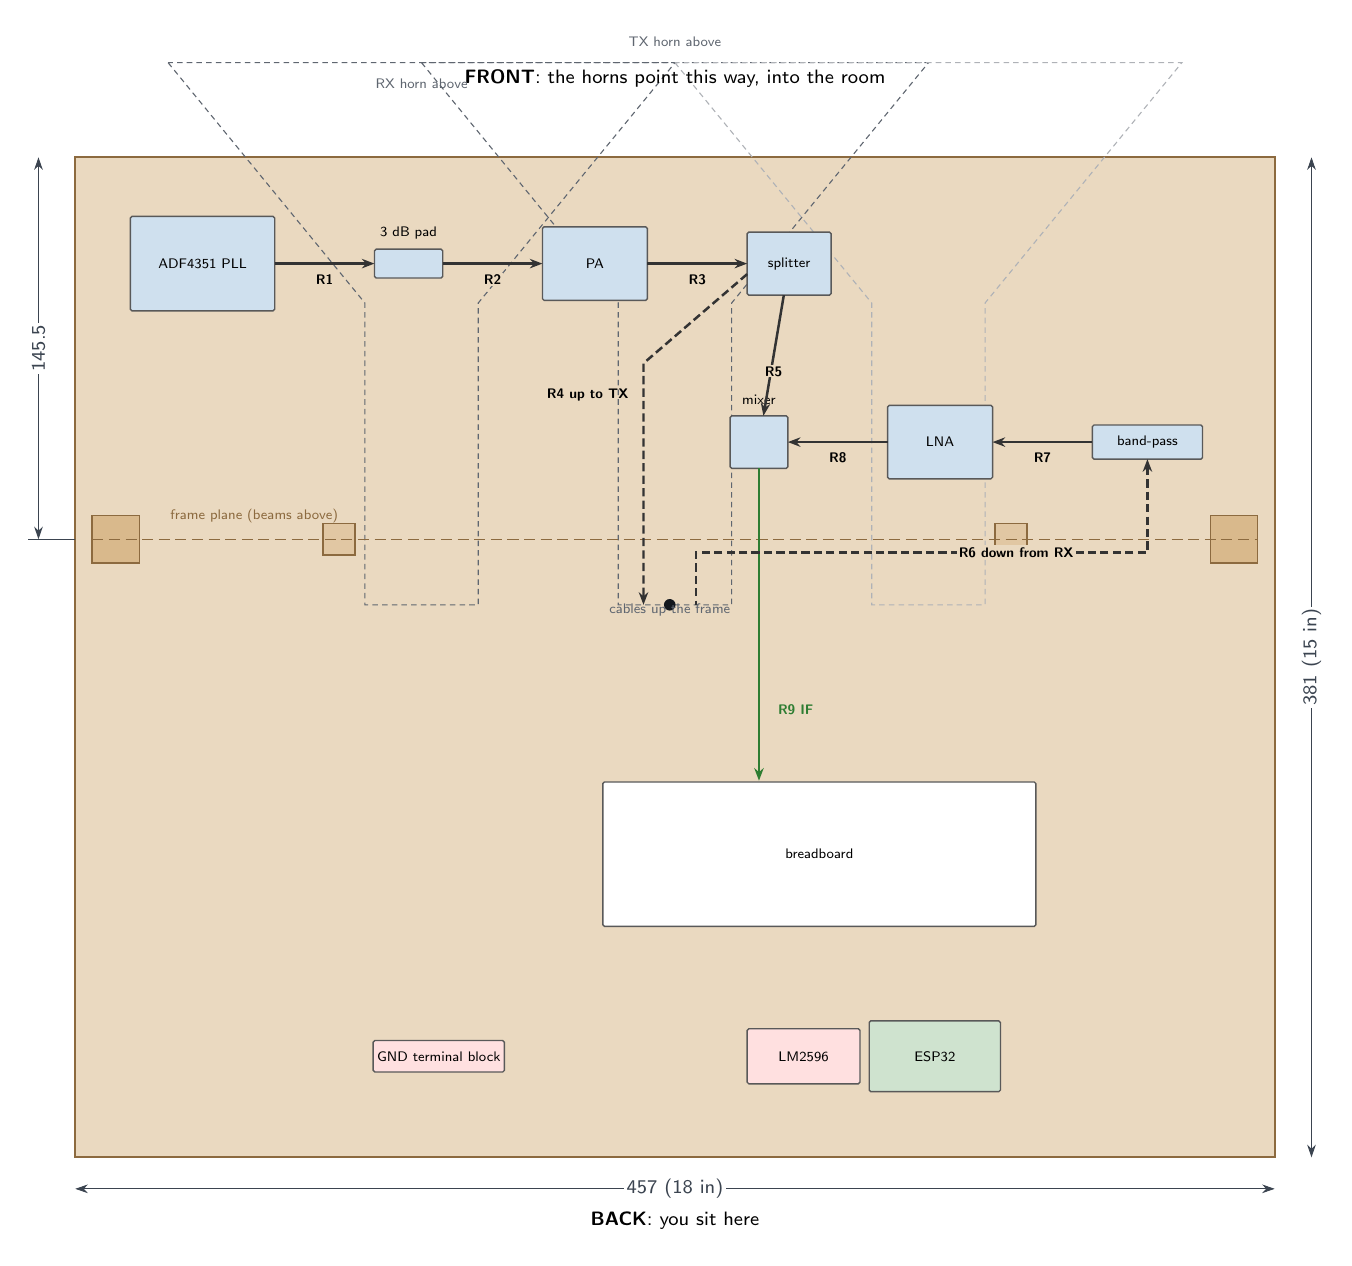
\begin{tikzpicture}[x=0.3333333333333333mm,y=0.3333333333333333mm,yscale=-1]
\path[woodpart,fill=wood!55] (-228.50,-190.50) rectangle (228.50,190.50);
\path[hidden] (-193.12,-226.55) -- (-118.15,-135.00) -- (-118.15,-20.00) -- (-74.95,-20.00) -- (-74.95,-135.00) -- (0.02,-226.55) -- cycle;
\path[hidden] (-96.57,-226.55) -- (-21.60,-135.00) -- (-21.60,-20.00) -- (21.60,-20.00) -- (21.60,-135.00) -- (96.57,-226.55) -- cycle;
\path[hidden,draw=muted!50] (-0.02,-226.55) -- (74.95,-135.00) -- (74.95,-20.00) -- (118.15,-20.00) -- (118.15,-135.00) -- (193.12,-226.55) -- cycle;
\node[font=\tiny,text=muted] at (-96.55,-218.55) {RX horn above};
\node[font=\tiny,text=muted] at (0.00,-234.55) {TX horn above};
\path[woodpart] (-222.00,-54.00) rectangle (-204.00,-36.00);
\path[woodpart,fill=wood!80] (-134.00,-51.00) rectangle (-122.00,-39.00);
\path[woodpart] (204.00,-54.00) rectangle (222.00,-36.00);
\path[woodpart,fill=wood!80] (122.00,-51.00) rectangle (134.00,-39.00);
\path[draw=woodedge,line width=0.4pt,dash pattern=on 4pt off 2pt] (-222.00,-45.00) -- (222.00,-45.00);
\node[font=\tiny,text=woodedge,anchor=west] at (-196.00,-54.00) {frame plane (beams above)};
\path[module,fill=rfmod] (-207.50,-168.00) rectangle (-152.50,-132.00);
\node[font=\tiny] at (-180.00,-150.00) {ADF4351 PLL};
\path[module,fill=rfmod] (-114.50,-155.50) rectangle (-88.50,-144.50);
\path[module,fill=rfmod] (-50.50,-164.00) rectangle (-10.50,-136.00);
\node[font=\tiny] at (-30.50,-150.00) {PA};
\path[module,fill=rfmod] (27.50,-162.00) rectangle (59.50,-138.00);
\node[font=\tiny] at (43.50,-150.00) {splitter};
\path[module,fill=rfmod] (159.00,-88.50) rectangle (201.00,-75.50);
\node[font=\tiny] at (180.00,-82.00) {band-pass};
\path[module,fill=rfmod] (81.00,-96.00) rectangle (121.00,-68.00);
\node[font=\tiny] at (101.00,-82.00) {LNA};
\path[module,fill=rfmod] (21.00,-92.00) rectangle (43.00,-72.00);
\path[module,fill=white] (-27.50,47.50) rectangle (137.50,102.50);
\node[font=\tiny] at (55.00,75.00) {breadboard};
\path[module,fill=pcb] (74.00,138.50) rectangle (124.00,165.50);
\node[font=\tiny] at (99.00,152.00) {ESP32};
\path[module,fill=red!12] (27.50,141.50) rectangle (70.50,162.50);
\node[font=\tiny] at (49.00,152.00) {LM2596};
\path[module,fill=red!12] (-115.00,146.00) rectangle (-65.00,158.00);
\node[font=\tiny] at (-90.00,152.00) {GND terminal block};
\node[font=\tiny] at (-101.50,-161.50) {3 dB pad};
\node[font=\tiny] at (32.00,-98.00) {mixer};
\path[draw=black!80,line width=0.9pt,-{Stealth[length=1.6mm]}] (-152.50,-150.00) -- (-114.50,-150.00);
\node[font=\tiny\bfseries,fill=wood!55,inner sep=0.5pt] at (-133.50,-144.00) {R1};
\path[draw=black!80,line width=0.9pt,-{Stealth[length=1.6mm]}] (-88.50,-150.00) -- (-50.50,-150.00);
\node[font=\tiny\bfseries,fill=wood!55,inner sep=0.5pt] at (-69.50,-144.00) {R2};
\path[draw=black!80,line width=0.9pt,-{Stealth[length=1.6mm]}] (-10.50,-150.00) -- (27.50,-150.00);
\node[font=\tiny\bfseries,fill=wood!55,inner sep=0.5pt] at (8.50,-144.00) {R3};
\path[draw=black!80,line width=0.9pt,-{Stealth[length=1.6mm]}] (41.47,-138.00) -- (33.69,-92.00);
\node[font=\tiny\bfseries,fill=wood!55,inner sep=0.5pt] at (37.58,-109.00) {R5};
\path[draw=black!80,line width=0.9pt,-{Stealth[length=1.6mm]}] (159.00,-82.00) -- (121.00,-82.00);
\node[font=\tiny\bfseries,fill=wood!55,inner sep=0.5pt] at (140.00,-76.00) {R7};
\path[draw=black!80,line width=0.9pt,-{Stealth[length=1.6mm]}] (81.00,-82.00) -- (43.00,-82.00);
\node[font=\tiny\bfseries,fill=wood!55,inner sep=0.5pt] at (62.00,-76.00) {R8};
\path[draw=sig,line width=0.9pt,-{Stealth[length=1.6mm]}] (32.00,-72.00) -- (32.00,47.00);
\node[font=\tiny\bfseries,text=sig] at (46.00,20.00) {R9 IF};
\path[draw=black!80,line width=0.9pt,dash pattern=on 3pt off 1.5pt,-{Stealth[length=1.6mm]}] (27.50,-146.00) -- (-12.00,-112.00) -- (-12.00,-20.00);
\node[font=\tiny\bfseries,anchor=east] at (-14.00,-100.00) {R4 up to TX};
\path[draw=black!80,line width=0.9pt,dash pattern=on 3pt off 1.5pt,{Stealth[length=1.6mm]}-] (180.00,-75.50) -- (180.00,-40.00) -- (8.00,-40.00) -- (8.00,-20.00);
\node[font=\tiny\bfseries,fill=wood!55,inner sep=0.8pt] at (130.00,-40.00) {R6 down from RX};
\fill[ink] (-2.00,-20.00) circle[radius=2.2];
\node[font=\tiny,text=muted,anchor=south] at (-2.00,-12.00) {cables up the frame};
\draw[dim] (-228.50,202.51) -- (228.50,202.51) node[dimlabel]{457 (18 in)};
\draw[dim] (242.51,-190.50) -- (242.51,190.50) node[dimlabel]{381 (15 in)};
\draw[dim] (-242.51,-190.50) -- (-242.51,-45.00) node[dimlabel]{145.5};
\path[ext] (-228.50,-45.00) -- (-246.50,-45.00);
\node[font=\scriptsize] at (0.00,-220.50) {\textbf{FRONT}: the horns point this way, into the room};
\node[font=\scriptsize] at (0.00,214.50) {\textbf{BACK}: you sit here};
\end{tikzpicture}

\caption{Top view of the board, 1\,:\,3: horns at the top, your seat at the bottom. Dashed outlines are the horns overhead. R1–R8 are the short SMA jumpers; R4 and R6 are the long runs to the horns.}\label{sec:plan}
\end{figure}

\newpage
\subsection{Cut list}
{\small
\begin{tabularx}{\linewidth}{@{}P{0.21\linewidth}p{8mm}P{0.24\linewidth}L@{}}
\toprule
\textbf{part} & \textbf{qty} & \textbf{stock} & \textbf{cut and drill} \\ \midrule
base board & 1 & 3/4\,in plywood & \boardW\,×\,\boardD\ (18\,×\,15\,in). Mark the centre line front to back \\
upright & 2 & 18\,mm (3/4\,in) square & \upH\ long, square ends. Pilot hole in the top end for the TX beam screw; one 3.5\,mm hole through at the RX beam \\
TX beam (top) & 1 & 12\,×\,32\,mm strip & \beamLen\ long. Two 3.5\,mm holes \upCC\ apart, centred; the TX saddle in the middle \\
RX beam (lower) & 1 & 12\,×\,32\,mm strip & \beamRXlen\ long, fits \emph{between} the uprights. Pilot holes in both ends; saddles at ±\,96.55 from centre \\
brace & 2 & 10\,mm dowel & about \braceLen\ long; both ends cut at \braceAngle° to the length (cut to fit) \\
saddle clamp & 3 & PETG print, or 3\,mm aluminium & page \pageref{sec:saddle} \\
foil screen & 1 & card + kitchen foil & \screenW\,×\,\screenH, foil side toward the horns \\
\bottomrule
\end{tabularx}}

\begin{note}[Why the beams join the way they do]
The 3-D model lets the beams pass through the uprights. Real wood cannot, so: the \textbf{TX beam sits on top} of both uprights, one screw down into each end; the \textbf{RX beam fits between them}, one screw in through each upright into its end. Both beam tops land exactly where the model puts them, \beamRXtop\ and \beamTXtop\ above the board. Each upright foot gets \textbf{two} L-brackets, one on its front face and one on its back, because the horns hang forward and pull the frame that way.
\end{note}

\subsection{Part drawings}
\begin{figure}[H]
\centering
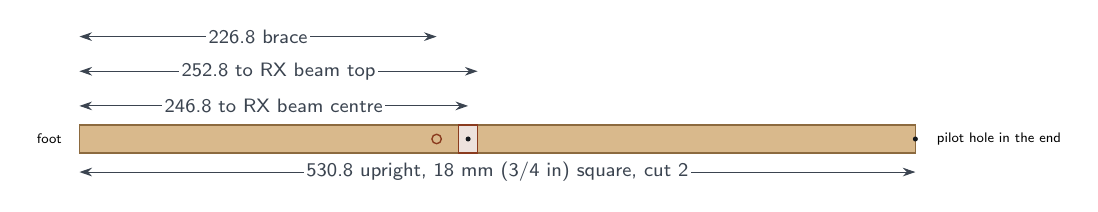
\begin{tikzpicture}[x=0.2mm,y=0.2mm]
\path[woodpart] (0,0) rectangle (530.80,18.00);
\path[draw=accent,line width=0.5pt,fill=accent!15] (240.80,0.00) rectangle (252.80,18.00);
\fill[ink] (246.80,9.00) circle[radius=1.6];
\fill[ink] (530.80,9.00) circle[radius=1.6];
\node[font=\tiny,anchor=west,xshift=1.5mm] at (530.80,9.00) {pilot hole in the end};
\path[draw=accent,line width=0.5pt] (226.80,9.00) circle[radius=3];
\draw[dim] (0.00,-11.99) -- (530.80,-11.99) node[dimlabel]{530.8 upright, 18 mm (3/4 in) square, cut 2};
\draw[dim] (0.00,30.01) -- (246.80,30.01) node[dimlabel]{246.8 to RX beam centre};
\draw[dim] (0.00,52.01) -- (252.80,52.01) node[dimlabel]{252.8 to RX beam top};
\draw[dim] (0.00,74.01) -- (226.80,74.01) node[dimlabel]{226.8 brace};
\node[font=\tiny,anchor=east,xshift=-1mm] at (0.00,9.00) {foot};
\end{tikzpicture}

\caption{Upright, 1\,:\,5, drawn lying down, foot to the left. The shaded band is where the RX beam end butts in.}
\end{figure}
\begin{figure}[H]
\centering
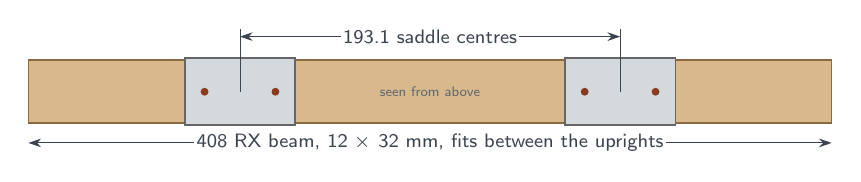
\begin{tikzpicture}[x=0.25mm,y=0.25mm]
\path[woodpart] (-204.00,0.00) rectangle (204.00,32.00);
\path[alupart,fill=alu!60] (-124.65,-1.00) rectangle (-68.45,33.00);
\fill[accent] (-114.55,16.00) circle[radius=2];
\fill[accent] (-78.55,16.00) circle[radius=2];
\path[alupart,fill=alu!60] (68.45,-1.00) rectangle (124.65,33.00);
\fill[accent] (78.55,16.00) circle[radius=2];
\fill[accent] (114.55,16.00) circle[radius=2];
\draw[dim] (-204.00,-9.99) -- (204.00,-9.99) node[dimlabel]{408 RX beam, 12 × 32 mm, fits between the uprights};
\draw[dim] (-96.55,44.01) -- (96.55,44.01) node[dimlabel]{193.1 saddle centres};
\path[ext] (-96.55,16.00) -- (-96.55,48.00);
\path[ext] (96.55,16.00) -- (96.55,48.00);
\node[font=\tiny,text=muted] at (0.00,16.00) {seen from above};
\end{tikzpicture}
\par\bigskip
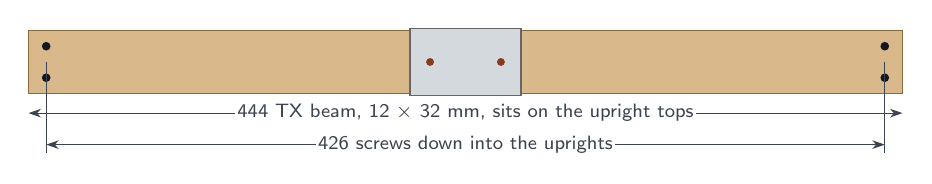
\begin{tikzpicture}[x=0.25mm,y=0.25mm]
\path[woodpart] (-222.00,0.00) rectangle (222.00,32.00);
\fill[ink] (-213.00,8.00) circle[radius=2.2];
\fill[ink] (-213.00,24.00) circle[radius=2.2];
\fill[ink] (213.00,8.00) circle[radius=2.2];
\fill[ink] (213.00,24.00) circle[radius=2.2];
\path[alupart,fill=alu!60] (-28.10,-1.00) rectangle (28.10,33.00);
\fill[accent] (-18.00,16.00) circle[radius=2];
\fill[accent] (18.00,16.00) circle[radius=2];
\draw[dim] (-222.00,-9.99) -- (222.00,-9.99) node[dimlabel]{444 TX beam, 12 × 32 mm, sits on the upright tops};
\draw[dim] (-213.00,-25.99) -- (213.00,-25.99) node[dimlabel]{426 screws down into the uprights};
\path[ext] (-213.00,16.00) -- (-213.00,-30.00);
\path[ext] (213.00,16.00) -- (213.00,-30.00);
\end{tikzpicture}

\caption{The two beams seen from above, 1\,:\,4. Grey are the saddle footprints, red the two screws that hold each saddle down.}
\end{figure}

\newpage
\subsection{The saddle clamp (full size)}\label{sec:saddle}
One per horn. The pipe drops into the U, narrow wall down, and two M4 screws through the cheeks pinch it. Centre the saddle on the beam and slide the horn until the saddle is \saddleBehind\,mm behind the throat (where the flare meets the pipe) — that puts all three mouths in one line.

\begin{figure}[H]
\centering
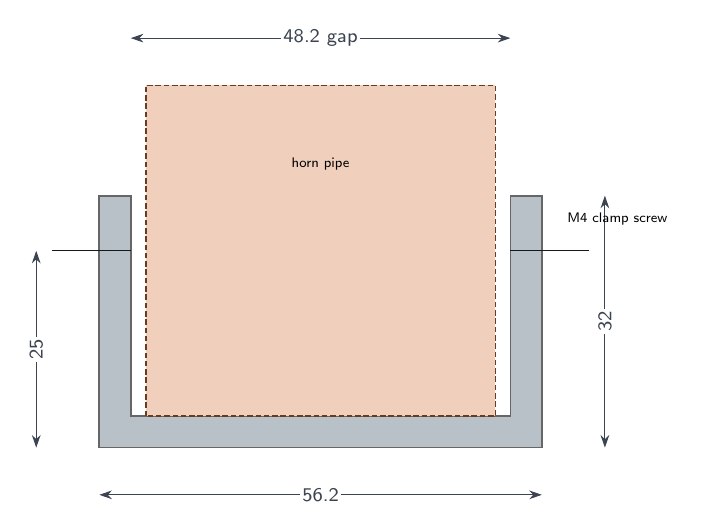
\begin{tikzpicture}[x=1.0mm,y=1.0mm]
\path[alupart] (-28.10,0.00) -- (28.10,0.00) -- (28.10,32.00) -- (24.10,32.00) -- (24.10,4.00) -- (-24.10,4.00) -- (-24.10,32.00) -- (-28.10,32.00) -- cycle;
\path[draw=cuedge,line width=0.6pt,fill=cuout!50,dash pattern=on 2pt off 1pt] (-22.20,4.00) rectangle (22.20,46.00);
\node[font=\tiny] at (0.00,36.00) {horn pipe};
\path[draw=ink,line width=0.4pt] (-24.10,25.00) -- (-34.10,25.00);
\path[draw=ink,line width=0.4pt] (24.10,25.00) -- (34.10,25.00);
\draw[dim] (-28.10,-5.99) -- (28.10,-5.99) node[dimlabel]{56.2};
\draw[dim] (-24.10,52.01) -- (24.10,52.01) node[dimlabel]{48.2 gap};
\draw[dim] (36.11,0.00) -- (36.11,32.00) node[dimlabel]{32};
\draw[dim] (-36.11,0.00) -- (-36.11,25.00) node[dimlabel]{25};
\node[font=\tiny,anchor=west] at (30.10,29.00) {M4 clamp screw};
\end{tikzpicture}

\caption{Saddle, front view at 1\,:\,1, \saddleD\,mm deep. 3-D print it in PETG at 40\,\% infill with the U opening upward, or bend it from 3\,mm aluminium strip. Holes: 4.5\,mm through both cheeks at the screw line; two 3.5\,mm holes in the base for wood screws into the beam.}
\end{figure}

\begin{warn}[Do not crush the pipe]
The inside of the pipe is what sets the horn's frequency. Line the cheeks with a strip of rubber or foam tape and tighten the clamp screws only until the horn will not slide. A dented pipe is a detuned horn.
\end{warn}

{\centering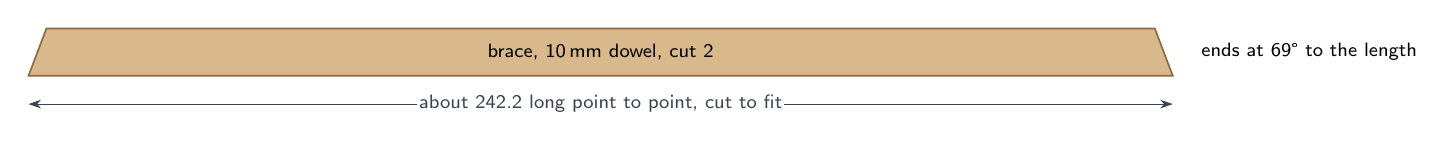
\begin{tikzpicture}[x=0.6mm,y=0.6mm,font=\scriptsize]
  \path[woodpart] (0,0) -- (\braceLen,0) -- ({\braceLen-3.8},10) -- (3.8,10) -- cycle;
  \draw[dim] (0,-6) -- (\braceLen,-6) node[dimlabel]{about \braceLen\ long point to point, cut to fit};
  \node at ({\braceLen/2},5) {brace, 10\,mm dowel, cut 2};
  \node[anchor=west] at ({\braceLen+4},5) {ends at \braceAngle° to the length};
\end{tikzpicture}\par}

\newpage
% ───────────────────────────────────────────────────────────── 5 the rf chain
\section{The RF chain}\label{sec:rf}

Seven bought modules, joined by SMA cables. There is nothing to make here; what matters is the order, the cable lengths, and that every connector is clean and tight. The modules go where the plan view on page \pageref{sec:plan} puts them: the transmit chain along the front edge, the receive chain behind it, so neither long cable has to cross the board.

\subsection{Cable runs}
{\small
\begin{tabularx}{\linewidth}{@{}p{7mm}P{0.25\linewidth}P{0.25\linewidth}p{14mm}L@{}}
\toprule
\textbf{run} & \textbf{from} & \textbf{to} & \textbf{cable} & \textbf{note} \\ \midrule
R1 & ADF4351, RF OUT A & 3\,dB pad & 20\,cm & the other ADF output: leave its cap on, or a 50\,Ω terminator \\
R2 & 3\,dB pad & PA (SPF5189Z \#1) IN & 20\,cm & or screw the pad straight onto the PA input \\
R3 & PA OUT & splitter S (input) & 20\,cm & \\
R4 & splitter port 1 & TX horn & \textbf{1\,m} & up the middle of the frame, tied every 10\,cm \\
R5 & splitter port 2 & mixer LO & 20\,cm & the LO must be +10 to +13\,dBm \\
R6 & RX horn & band-pass IN & \textbf{60\,cm} & down the middle of the frame, then right along the board. If 60\,cm will not reach, 1\,m costs only 0.5\,dB \\
R7 & band-pass OUT & LNA (SPF5189Z \#2) IN & 20\,cm & \\
R8 & LNA OUT & mixer RF & 20\,cm & \\
R9 & mixer IF & breadboard J1 & pigtail & SMA to two bare leads: centre to J1 pin 1, braid to pin 2 \\
\bottomrule
\end{tabularx}}

\begin{note}[SMA connectors in one paragraph]
Turn the nut, never the cable body. Finger tight, then an eighth of a turn with the spanner: that is all an SMA wants. Over-tightening splits the centre pin. Look into each connector before mating it; a bent pin or a fleck of solder in one ruins every measurement after it. Bend cables no tighter than a 2\,cm radius.
\end{note}

\subsection{Module power}
The ADF4351, the PA and the LNA each take 5\,V from the breadboard through their own ferrite bead and capacitors: J6, J7 and J8. Use red and black 22\,AWG, twisted together, and keep them short. The mixer, splitter, pad and filter are passive and take no power.

{\small
\begin{tabularx}{\linewidth}{@{}P{0.2\linewidth}P{0.13\linewidth}P{0.2\linewidth}L@{}}
\toprule
\textbf{module} & \textbf{supply} & \textbf{from} & \textbf{note} \\ \midrule
ADF4351 PLL & 5\,V, ~120\,mA & J6 (through FB1) & logic is 3.3\,V; the ESP32 drives it directly through 33\,Ω \\
PA, SPF5189Z \#1 & 5\,V, ~90\,mA & J7 (through FB2) & gets warm: that is normal \\
LNA, SPF5189Z \#2 & 5\,V, ~90\,mA & J8 (through FB3) & identical board to the PA \\
ESP32 & USB & the laptop & also its serial link \\
\bottomrule
\end{tabularx}}

\newpage
% ───────────────────────────────────────────────────────────── 6 schematics
\section{The electronics, as schematics}\label{sec:sch}

Everything on the breadboard, redrawn as five small circuits. The reference numbers (R1, C9, J2…) match the breadboard layout, the pick list and the assembly steps. The op-amps run from a single +12\,V supply, so instead of ground the signal swings around \textbf{VREF}, a steady half-supply point made in figure~\ref{fig:vref}.

\begin{figure}[H]
\centering
\begin{circuitikz}[scale=0.9,transform shape,font=\footnotesize]
  \ctikzset{resistors/scale=0.7,capacitors/scale=0.7}
  % ── row 1: IF input and the two gain stages
  \draw (0,0) node[ocirc]{} node[left,align=right]{J1\\IF in} -- (1.2,0);
  \draw (1.2,0) node[circ]{} to[R,l_={R1 49.9\,Ω}] (1.2,-2) node[ground]{};
  \draw (1.2,0) -- (3.0,0) node[circ]{} to[C,l_={C20 1n}] (3.0,-2) node[ground]{};
  \draw (3.0,0) to[C,l=C1,a_=100n film] (4.8,0) node[circ]{};
  \draw (4.8,0) to[R,l_=R2,a^=10k] (4.8,-2) node[below]{VREF};
  \node[op amp,noinv input down,anchor=+] (A) at (5.8,0) {\scriptsize U1A};
  \draw (4.8,0) -- (A.+);
  \draw (A.-) -- ++(-0.4,0) coordinate(an) -- ++(0,1.3) coordinate(at);
  \draw (at) node[circ]{} to[R,l=R3,a_=100k] (at -| A.out) -- (A.out);
  \draw (at) to[R,l_=R4,a^=1k] ++(-2.0,0) node[left]{VREF};
  \draw (A.out) node[circ]{} to[C,l=C2,a_=100n film] ++(1.9,0) coordinate(bp) node[circ]{};
  \draw (bp) to[R,l_=R6,a^=10k] ++(0,-2) node[below]{VREF};
  \node[op amp,noinv input down,anchor=+] (B) at ($(bp)+(1,0)$) {\scriptsize U1B};
  \draw (bp) -- (B.+);
  \draw (B.-) -- ++(-0.4,0) -- ++(0,1.3) coordinate(bt);
  \draw (bt) node[circ]{} to[R,l=R7,a_=10k] (bt -| B.out) -- (B.out);
  \draw (bt) to[R,l_=R8,a^=1k] ++(-2.0,0) node[left]{VREF};
  \draw (B.out) node[circ]{} -- ++(0.6,0) node[ocirc]{} node[right]{\textbf{X}};
  \node[font=\scriptsize,text=muted,align=center] at ($(A.out)+(-1.2,-1.5)$) {gain 101};
  \node[font=\scriptsize,text=muted,align=center] at ($(B.out)+(-1.2,-1.5)$) {gain 11};
  % ── row 2: anti-alias filter, buffer, output
  \begin{scope}[yshift=-4.8cm]
  \draw (0,0) node[ocirc]{} node[left]{\textbf{X}} to[R,l=R12,a_=1k] (2,0) node[circ]{};
  \draw (2,0) to[C,l_=C9,a^=10n] (2,-2) node[below]{VREF};
  \node[op amp,noinv input down,anchor=+] (C) at (3,0) {\scriptsize U2B};
  \draw (2,0) -- (C.+);
  \draw (C.-) -- ++(-0.4,0) -- ++(0,1.0) coordinate(ct) -- (ct -| C.out) -- (C.out);
  \draw (C.out) node[circ]{} to[R,l=R13,a_=100\,Ω] ++(2,0) to[eC,l=C10,a_=10µ] ++(2,0) coordinate(o) node[circ]{};
  \draw (o) to[R,l_=R14,a^=100k] ++(0,-2) node[ground]{};
  \draw (o) -- ++(1.2,0) node[ocirc]{} node[right,align=left]{J2 AUDIO L\\to UMC404HD IN 1};
  \node[font=\scriptsize,text=muted,align=center] at ($(C.out)+(-0.9,-1.4)$) {buffer};
  \node[font=\scriptsize,text=muted,align=left,anchor=west] at (1.0,-3.1) {R12 + C9: cut-off 15.9\,kHz};
  \end{scope}
\end{circuitikz}
\caption{The beat-tone amplifier. R1 is the mixer's 50\,Ω load. C1 and C2 block DC and roll off below about 160\,Hz, where the leakage and the room's clutter live; they \emph{must} be film capacitors. Total gain 101\,×\,11 = 1111, or 61\,dB. U2B buffers the filter so the sound card's input cannot load it; C10 removes the DC so the output sits at 0\,V.}\label{fig:amp}
\end{figure}

\begin{figure}[H]
\centering
\begin{minipage}[b]{0.47\linewidth}\centering
\begin{circuitikz}[scale=0.85,transform shape,font=\footnotesize]
  \ctikzset{resistors/scale=0.7,capacitors/scale=0.7}
  \draw (0,3) node[above]{VANA} to[R,l_=R9,a^=10k] (0,1) node[circ]{} to[R,l_=R10,a^=10k] (0,-1) node[ground]{};
  \draw (0,1) -- (2.0,1) node[circ]{} to[eC,l_=C5,a^=10µ] (2.0,-1) node[ground]{};
  \node[op amp,noinv input down,anchor=+] (V) at (3.0,1) {\scriptsize U2A};
  \draw (2.0,1) -- (V.+);
  \draw (V.-) -- ++(-0.4,0) -- ++(0,0.9) coordinate(vt) -- (vt -| V.out) -- (V.out);
  \draw (V.out) node[circ]{} to[R,l=R11,a_=47\,Ω] ++(1.8,0) coordinate(vr) node[circ]{};
  \draw (vr) to[eC,l_=C6,a^=47µ] ++(0,-2) node[ground]{};
  \draw (vr) -- ++(0.6,0) node[right]{VREF};
\end{circuitikz}
\caption{VREF, the half-supply reference: half of VANA, about 5.8\,V.}\label{fig:vref}
\end{minipage}\hfill
\begin{minipage}[b]{0.5\linewidth}\centering
\begin{circuitikz}[scale=0.85,transform shape,font=\footnotesize]
  \ctikzset{resistors/scale=0.7,capacitors/scale=0.7}
  \draw (0,0) node[ocirc]{} node[left]{ESP32 GPIO25 SYNC} to[R,l=R23,a_=10k] (2.4,0) node[circ]{};
  \draw (2.4,0) to[R,l_=R24,a^=1k] (2.4,-2) node[ground]{};
  \draw (2.4,0) -- (3.4,0) node[ocirc]{} node[right,align=left]{J12 AUDIO R\\to IN 2};
\end{circuitikz}
\caption{The sync divider: the ESP32's 3.3\,V chirp marker cut to 0.3\,V, a safe line level.}\label{fig:sync}
\end{minipage}
\end{figure}

\begin{figure}[H]
\centering
\begin{circuitikz}[scale=0.85,transform shape,font=\footnotesize]
  \ctikzset{resistors/scale=0.7,capacitors/scale=0.7,diodes/scale=0.7}
  \draw (0,0) node[ocirc]{} node[left,align=right]{J3\\12\,V in} to[D*,l=D1,a_=1N5822] (2.4,0) node[circ]{} coordinate(vp);
  \draw (vp) node[above=8pt]{VPROT} to[eC,l_=C11,a^=100µ] ++(0,-2) node[ground]{};
  \draw (vp) -- (3.8,0) node[circ]{} coordinate(j4);
  \draw (j4) -- ++(0,1.4) node[ocirc]{} node[above,align=center]{J4 to LM2596 IN};
  \draw (j4) to[R,l=R15,a_=10\,Ω] (6.2,0) node[circ]{} coordinate(va);
  \draw (va) to[eC,l_=C13,a^=100µ] ++(0,-2) node[ground]{};
  \draw (va) -- ++(1.2,0) node[right,align=left]{\textbf{VANA}, op-amp supply\\(+ C3, C7 100n at the\\op-amp pins)};
  \begin{scope}[yshift=-4.4cm]
  \draw (0,0) node[ocirc]{} node[left,align=right]{J5\\5\,V from\\LM2596} -- (1.6,0) node[circ]{} coordinate(v5);
  \draw (v5) to[eC,l_={C12 100µ}] ++(0,-2) node[ground]{};
  \draw (v5) -- (12.8,0);
  \foreach \x/\fb/\ce/\cc/\j/\who in {3.0/FB1/C14/C15/J6/ADF4351, 7.9/FB2/C16/C17/J7/PA, 12.8/FB3/C18/C19/J8/LNA}{
    \draw (\x,0) node[circ]{} to[L,l_=\fb] (\x,-1.8) coordinate(m);
    \draw (m) -- ++(1.0,0) node[circ]{} coordinate(m1) to[eC,l_={\ce\ 10µ}] ++(0,-1.8) node[ground]{};
    \draw (m1) -- ++(1.9,0) node[circ]{} coordinate(m2) to[C,l_={\cc\ 100n}] ++(0,-1.8) node[ground]{};
    \draw (m2) -- ++(1.0,0) node[ocirc]{} node[below=2pt,align=center,font=\scriptsize]{\j\\\who};
  }
  \end{scope}
\end{circuitikz}
\caption{Power. D1 blocks a backwards supply. VPROT feeds the buck converter and, through R15, the op-amps (VANA). The buck's 5\,V goes to each RF module through its own ferrite bead and a 10\,µ + 100\,n pair, so their noise stays out of each other.}\label{fig:power}
\end{figure}

\begin{figure}[H]
\centering
\begin{circuitikz}[scale=0.85,transform shape,font=\footnotesize]
  \ctikzset{resistors/scale=0.65}
  \node[draw,fill=pcb,minimum width=22mm,minimum height=62mm,align=center] (esp) at (0,0) {\textbf{ESP32}\\radar\_ctl};
  \node[draw,fill=rfmod,minimum width=22mm,minimum height=50mm,align=center] (adf) at (8.6,0.6) {\textbf{ADF4351}};
  \foreach \y/\g/\r/\p in {2.6/18/R16/CLK, 1.6/23/R17/DATA, 0.6/5/R18/LE}{
    \draw (esp.east |- 0,\y) node[left,font=\scriptsize]{GPIO\g} -- ++(0.8,0) to[R,l={\r\ 33\,Ω}] ++(2.2,0) -- (adf.west |- 0,\y) node[right,font=\scriptsize]{\p};
  }
  \draw (esp.east |- 0,-0.4) node[left,font=\scriptsize]{GPIO19} -- (adf.west |- 0,-0.4) node[right,font=\scriptsize]{LD};
  \draw (adf.west |- 0,-1.2) coordinate(ce) node[right,font=\scriptsize]{CE};
  \draw (ce) -- ++(-1.2,0) coordinate(cen) node[circ]{} to[R,l_=R19,a^=10k] ++(0,-1.6) node[ground]{};
  \draw (cen) -- ++(-1.4,0) node[ocirc]{} node[left,align=right,font=\scriptsize]{JP3 to 3V3\\(cap on = enabled)};
  \draw (esp.east |- 0,-2.2) node[left,font=\scriptsize]{GPIO25} -- ++(1.0,0) node[right,font=\scriptsize]{SYNC $\rightarrow$ figure \ref{fig:sync}};
  \draw (esp.east |- 0,-2.8) node[left,font=\scriptsize]{3V3} -- ++(1.0,0) node[right,font=\scriptsize]{to JP3, J11};
  \draw (esp.west |- 0,-2.8) node[right,font=\scriptsize]{GND} -- ++(-0.8,0) node[ground]{};
  \draw (esp.west |- 0,2.2) node[right,font=\scriptsize]{USB} -- ++(-0.9,0) node[left,font=\scriptsize]{laptop};
  \node[font=\scriptsize,text=muted,align=left,anchor=north west] at (-1.2,-3.6) {Optional turntable (stage 2): GPIO26 STEP, GPIO27 DIR, GPIO14 EN to the A4988 on J11,\\with R21, R22 10k pull-downs on STEP and DIR and R20 10k pull-up on EN (keeps the motor off at boot).};
\end{circuitikz}
\caption{The logic wiring. The 33\,Ω resistors soften the clock edges so they do not ring on the 15\,cm leads. Lock detect (LD) comes back to GPIO19 so the firmware can report \code{lock:1}.}\label{fig:logic}
\end{figure}

\newpage
% ───────────────────────────────────────────────────────────── 7 breadboard
\section{The breadboard}\label{sec:bb}

The circuits above, laid out on one 830-point breadboard. Signal flows left to right: the IF comes in at column 2, the amplified beat leaves at column 36; power enters bottom left, the module 5\,V leaves at columns 38–45, the logic sits at the right. Part 2 builds it in seventeen steps, each with its own picture.

\begin{figure}[H]
\centering
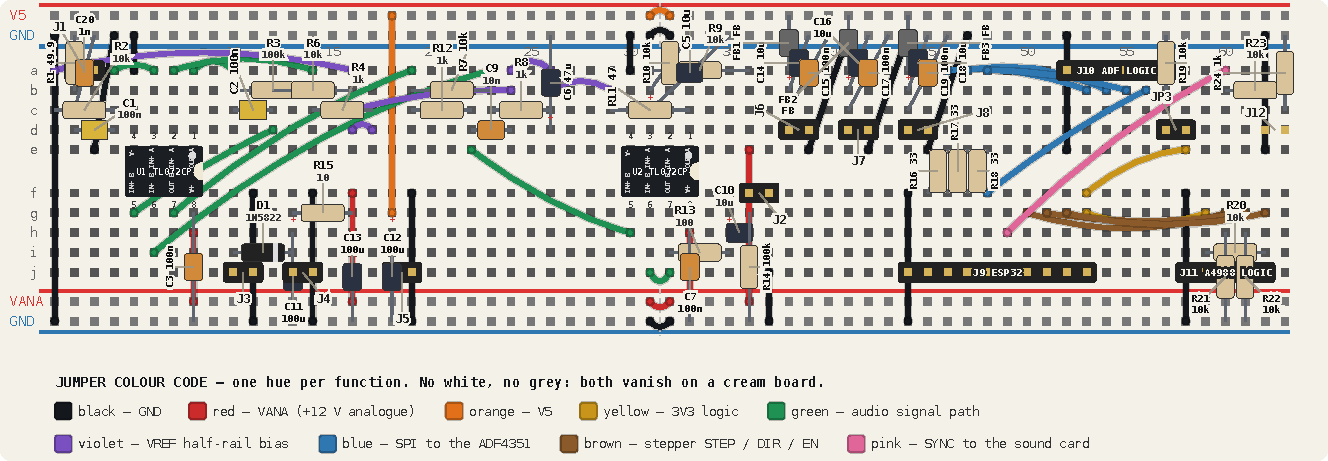
\includegraphics[width=\linewidth]{breadboard.pdf}
\caption{The finished breadboard. Columns 1–63 left to right; rows a–e on top, f–j below. Rails: top red 5\,V, top blue GND, bottom red VANA (12\,V analogue), bottom blue GND.}
\end{figure}

\subsection{The jumper colour code}\label{sec:colours}
One colour per job, so a wire in the wrong place stands out. Nothing electrical depends on it; if your kit is short of a colour, substitute one and note it here.

{\small
\begin{tabularx}{\linewidth}{@{}p{8mm}P{0.13\linewidth}P{0.2\linewidth}p{12mm}L@{}}
\toprule
& \textbf{colour} & \textbf{carries} & \textbf{wires} & \\ \midrule
\tikz\fill[black] (0,0) rectangle (5mm,2.5mm); & black & GND & 17 & \\
\tikz\fill[red!80!black] (0,0) rectangle (5mm,2.5mm); & red & VANA, 12\,V analogue & 5 & \\
\tikz\fill[orange] (0,0) rectangle (5mm,2.5mm); & orange & 5\,V & 2 & \\
\tikz\fill[yellow!90!black] (0,0) rectangle (5mm,2.5mm); & yellow & 3V3 logic & 2 & \\
\tikz\fill[green!60!black] (0,0) rectangle (5mm,2.5mm); & green & audio signal path & 9 & \\
\tikz\fill[violet] (0,0) rectangle (5mm,2.5mm); & violet & VREF half-rail & 5 & \\
\tikz\fill[blue!80!black] (0,0) rectangle (5mm,2.5mm); & blue & SPI to the ADF4351 & 4 & \\
\tikz\fill[brown] (0,0) rectangle (5mm,2.5mm); & brown & stepper STEP/DIR/EN & 3 & \\
\tikz\fill[pink] (0,0) rectangle (5mm,2.5mm); & pink & SYNC & 1 & \\
\bottomrule
\end{tabularx}}

There is deliberately no white or grey wire: on a cream breadboard both disappear.

\subsection{Pick list}\label{sec:picklist}
Grouped by value, with how many to take from the drawer. \textbf{Bold} values set a gain, a cut-off or a termination: do not substitute those.

{\small
\begin{longtable}{@{}P{0.12\linewidth}p{9mm}p{9mm}P{0.43\linewidth}P{0.24\linewidth}@{}}
\toprule
\textbf{value} & \textbf{need} & \textbf{take} & \textbf{substitute?} & \textbf{refs} \\ \midrule
\endhead
\rowsfrom{picklist_rows}
\multicolumn{5}{l}{\rule{0pt}{11pt}\textbf{\color{accent}Also}}\\
4.7k & 1 & 2 & for R4 on first power-up only (gain 22 instead of 101) & R4 \\
header strip & 41 pins & 2 strips & 0.1\,in male, snapped into 2-, 5-, 6- and 10-pin lengths & J1–J12, JP3 \\
\bottomrule
\end{longtable}}

\subsection{Connectors}
Every wire that leaves the breadboard lands on a header. The holes column gives pin 1 first: on J12, pin 1 is the right-hand one.

{\small
\begin{longtable}{@{}p{9mm}P{0.13\linewidth}P{0.33\linewidth}P{0.42\linewidth}@{}}
\toprule
\textbf{ref} & \textbf{holes} & \textbf{pins} & \textbf{goes to} \\ \midrule
\endhead
J1 & a2, a3 & 1 IF, 2 GND & mixer IF via the R9 pigtail \\
J2 & f36, f37 & 1 AUDIO\_L, 2 GND & UMC404HD INPUT 1, 1/4\,in TS cable \\
J3 & j10, j11 & 1 +12\,V, 2 GND & the 12\,V supply \\
J4 & j13, j14 & 1 VPROT, 2 GND & LM2596 IN+ / IN− \\
J5 & j18, j19 & 1 5\,V, 2 GND & LM2596 OUT+ / OUT− \\
J6 & d38, d39 & 1 5\,V, 2 GND & ADF4351 VCC / GND \\
J7 & d41, d42 & 1 5\,V, 2 GND & PA module + / − \\
J8 & d44, d45 & 1 5\,V, 2 GND & LNA module + / − \\
J9 & j44–j53 & 1 GND, 2 SCK, 3 MOSI, 4 LE, 5 LD, 6 SYNC, 7 STEP, 8 DIR, 9 EN, 10 3V3 & ESP32: GND, D18, D23, D5, D19, D25, D26, D27, D14, 3V3 \\
J10 & a52–a57 & 1 GND, 2 CLK, 3 DATA, 4 LE, 5 LD, 6 CE & ADF4351 logic header, \emph{by silkscreen name}: the boards differ in pin order \\
JP3 & d57, d58 & 1 CE, 2 3V3 & a jumper cap: on = PLL enabled \\
J11 & j58–j62 & 1 GND, 2 3V3, 3 STEP, 4 DIR, 5 EN & A4988, optional, stage 2 \\
J12 & d63, d62 & 1 AUDIO\_R, 2 GND & UMC404HD INPUT 2 (stage 1), 1/4\,in TS cable \\
\bottomrule
\end{longtable}}

\end{document}
